\chapter{Kết quả thực nghiệm bổ sung}
\label{app:chapter4_draft}

Phụ lục này lưu các đồ thị chi tiết ở cấp một hạt giống và các phân phối OOD theo từng kịch bản. Các hình một hạt giống không được dùng thay cho giá trị trung bình ba hạt giống trong phần kết quả chính; mục đích của chúng là minh họa hình dạng đường cong, hiệu chuẩn và cấu trúc biểu diễn.

\section{Đường cong ROC, Precision--Recall và hiệu chuẩn}

\begin{table}[H]
\centering
\small
\begin{tabular}{|l|c|c|c|c|c|c|}
\hline
\textbf{Dữ liệu} & \textbf{Seed} & \textbf{Macro-AUROC} & \textbf{Micro-AUROC} & \textbf{Macro-AUPRC} & \textbf{Micro-AUPRC} & \textbf{ECE} \\ \hline
CTCH & 42 & 0,9603 & 0,9559 & 0,6131 & 0,5747 & 0,2210 \\ \hline
BTXRD & 123 & 0,8899 & 0,9562 & 0,6099 & 0,8387 & 0,0781 \\ \hline
\end{tabular}
\caption{Giá trị đi kèm các đường cong minh họa ở cấp một hạt giống}
\label{tab:app_ch4_single_seed_curves}
\end{table}

\begin{figure}[H]
\centering
\begin{subfigure}[t]{0.49\textwidth}
\centering
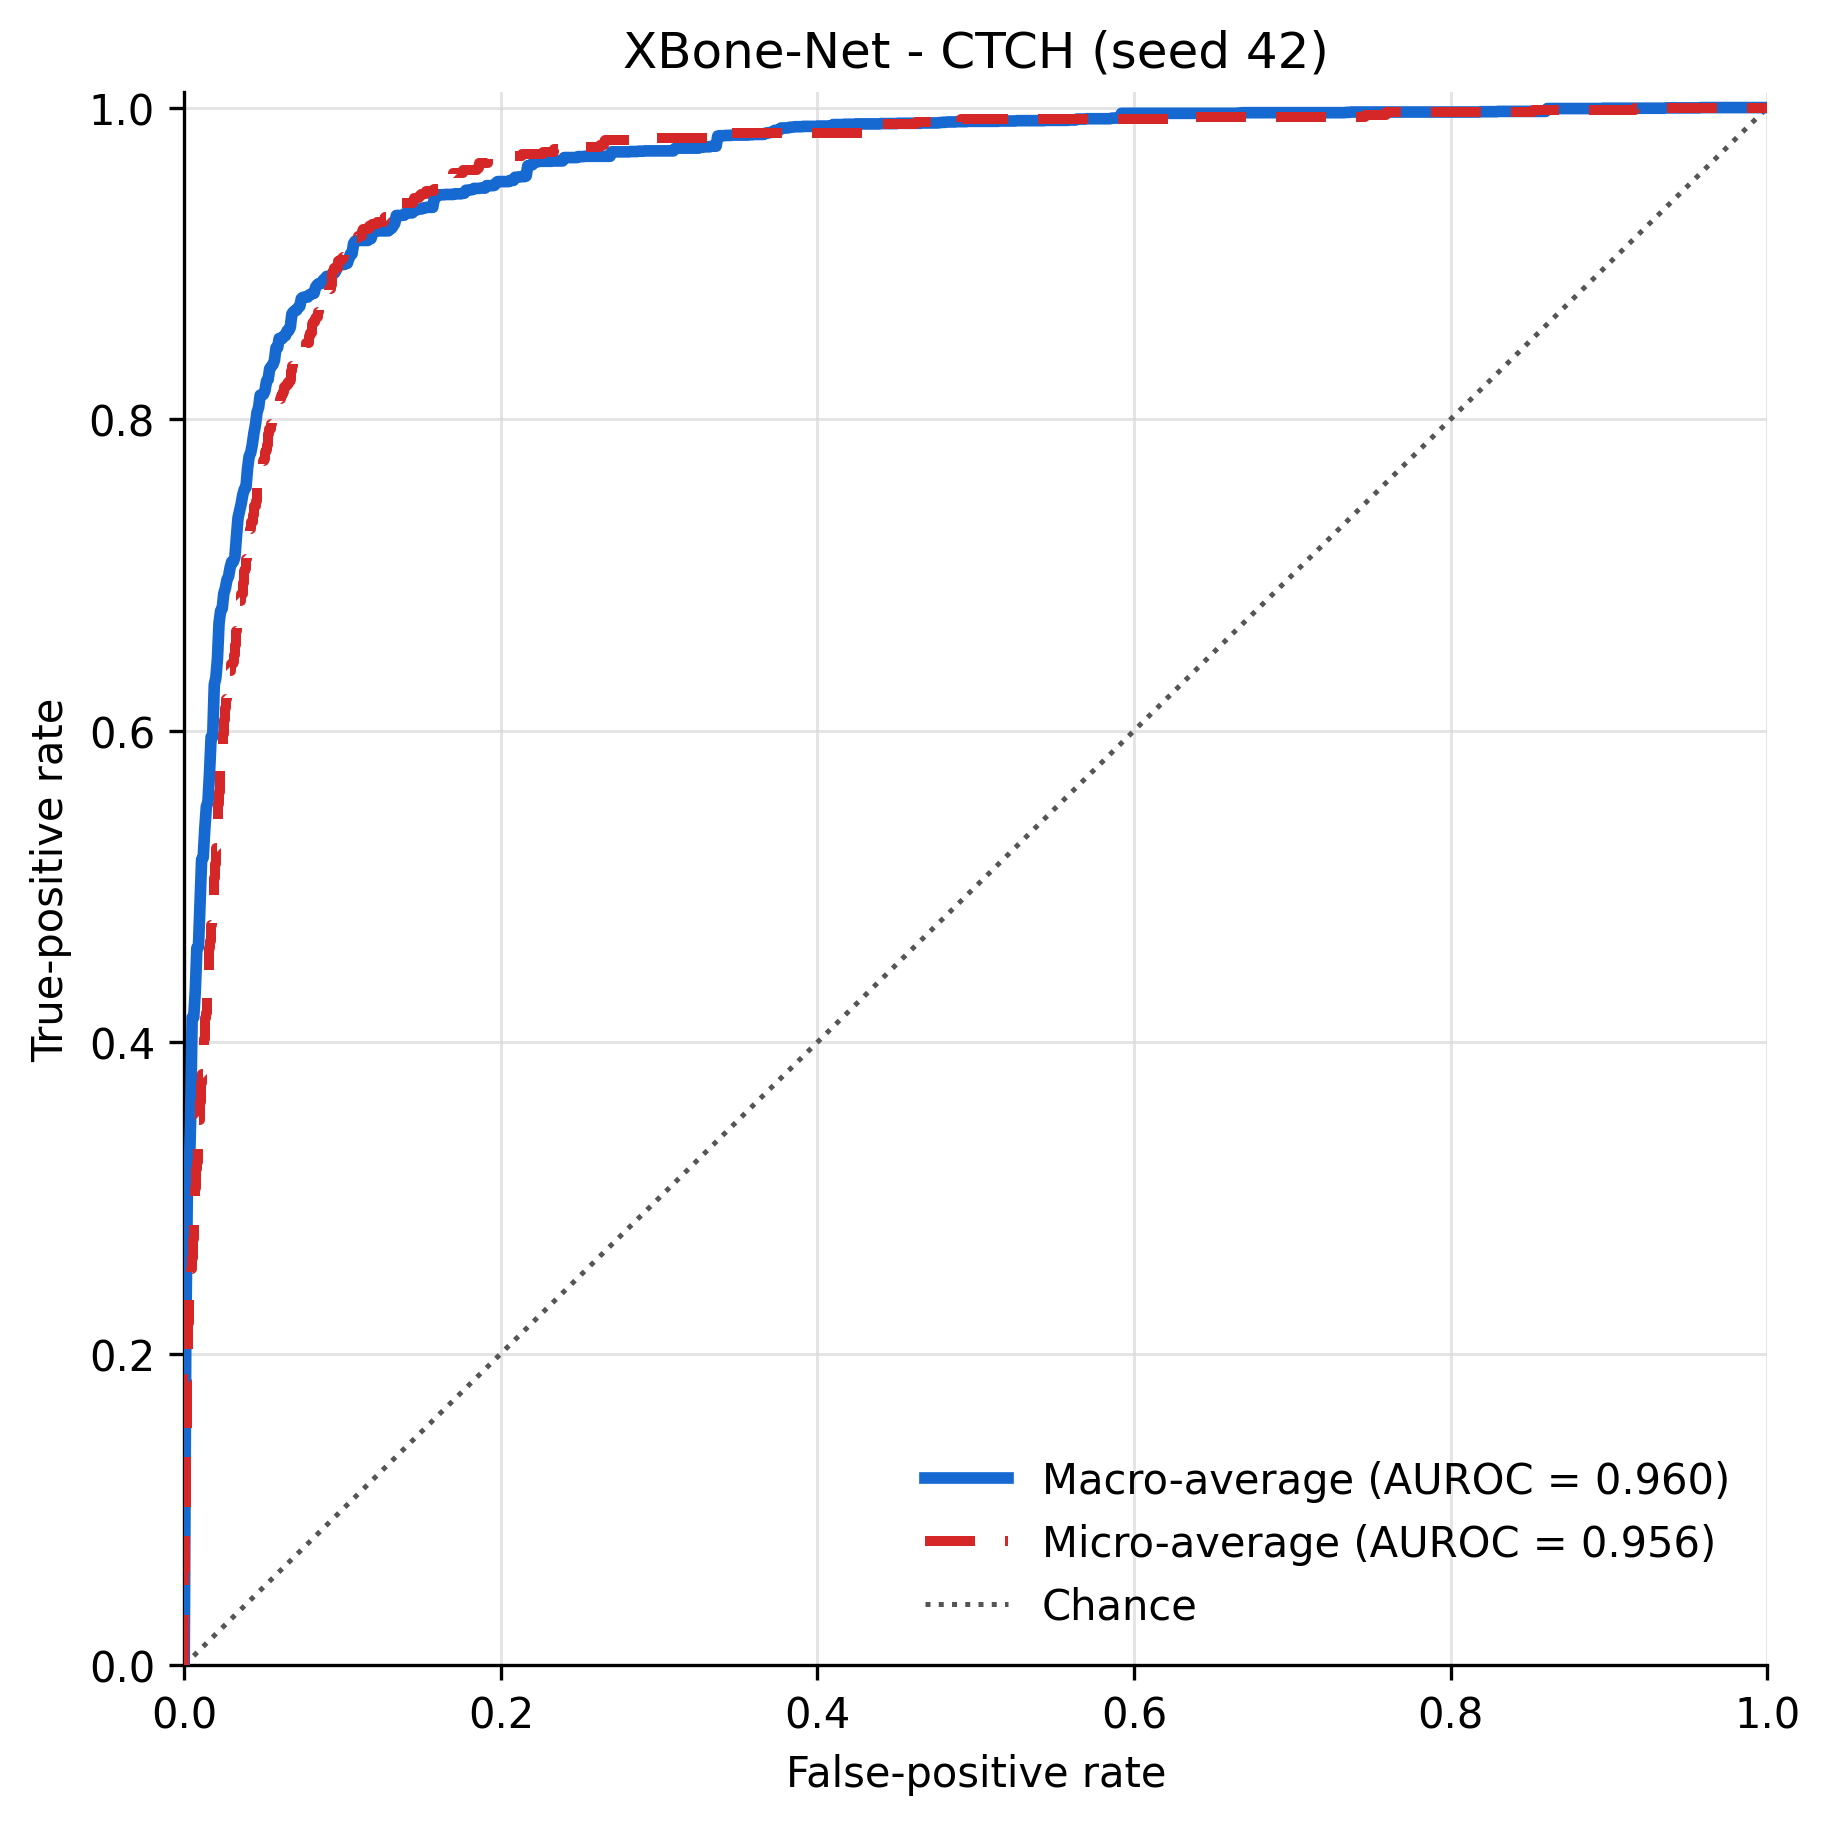
\includegraphics[width=\textwidth]{images/chapter4_draft/appendix/roc_ctch_seed42.png}
\caption{ROC trên CTCH, seed 42}
\end{subfigure}
\hfill
\begin{subfigure}[t]{0.49\textwidth}
\centering
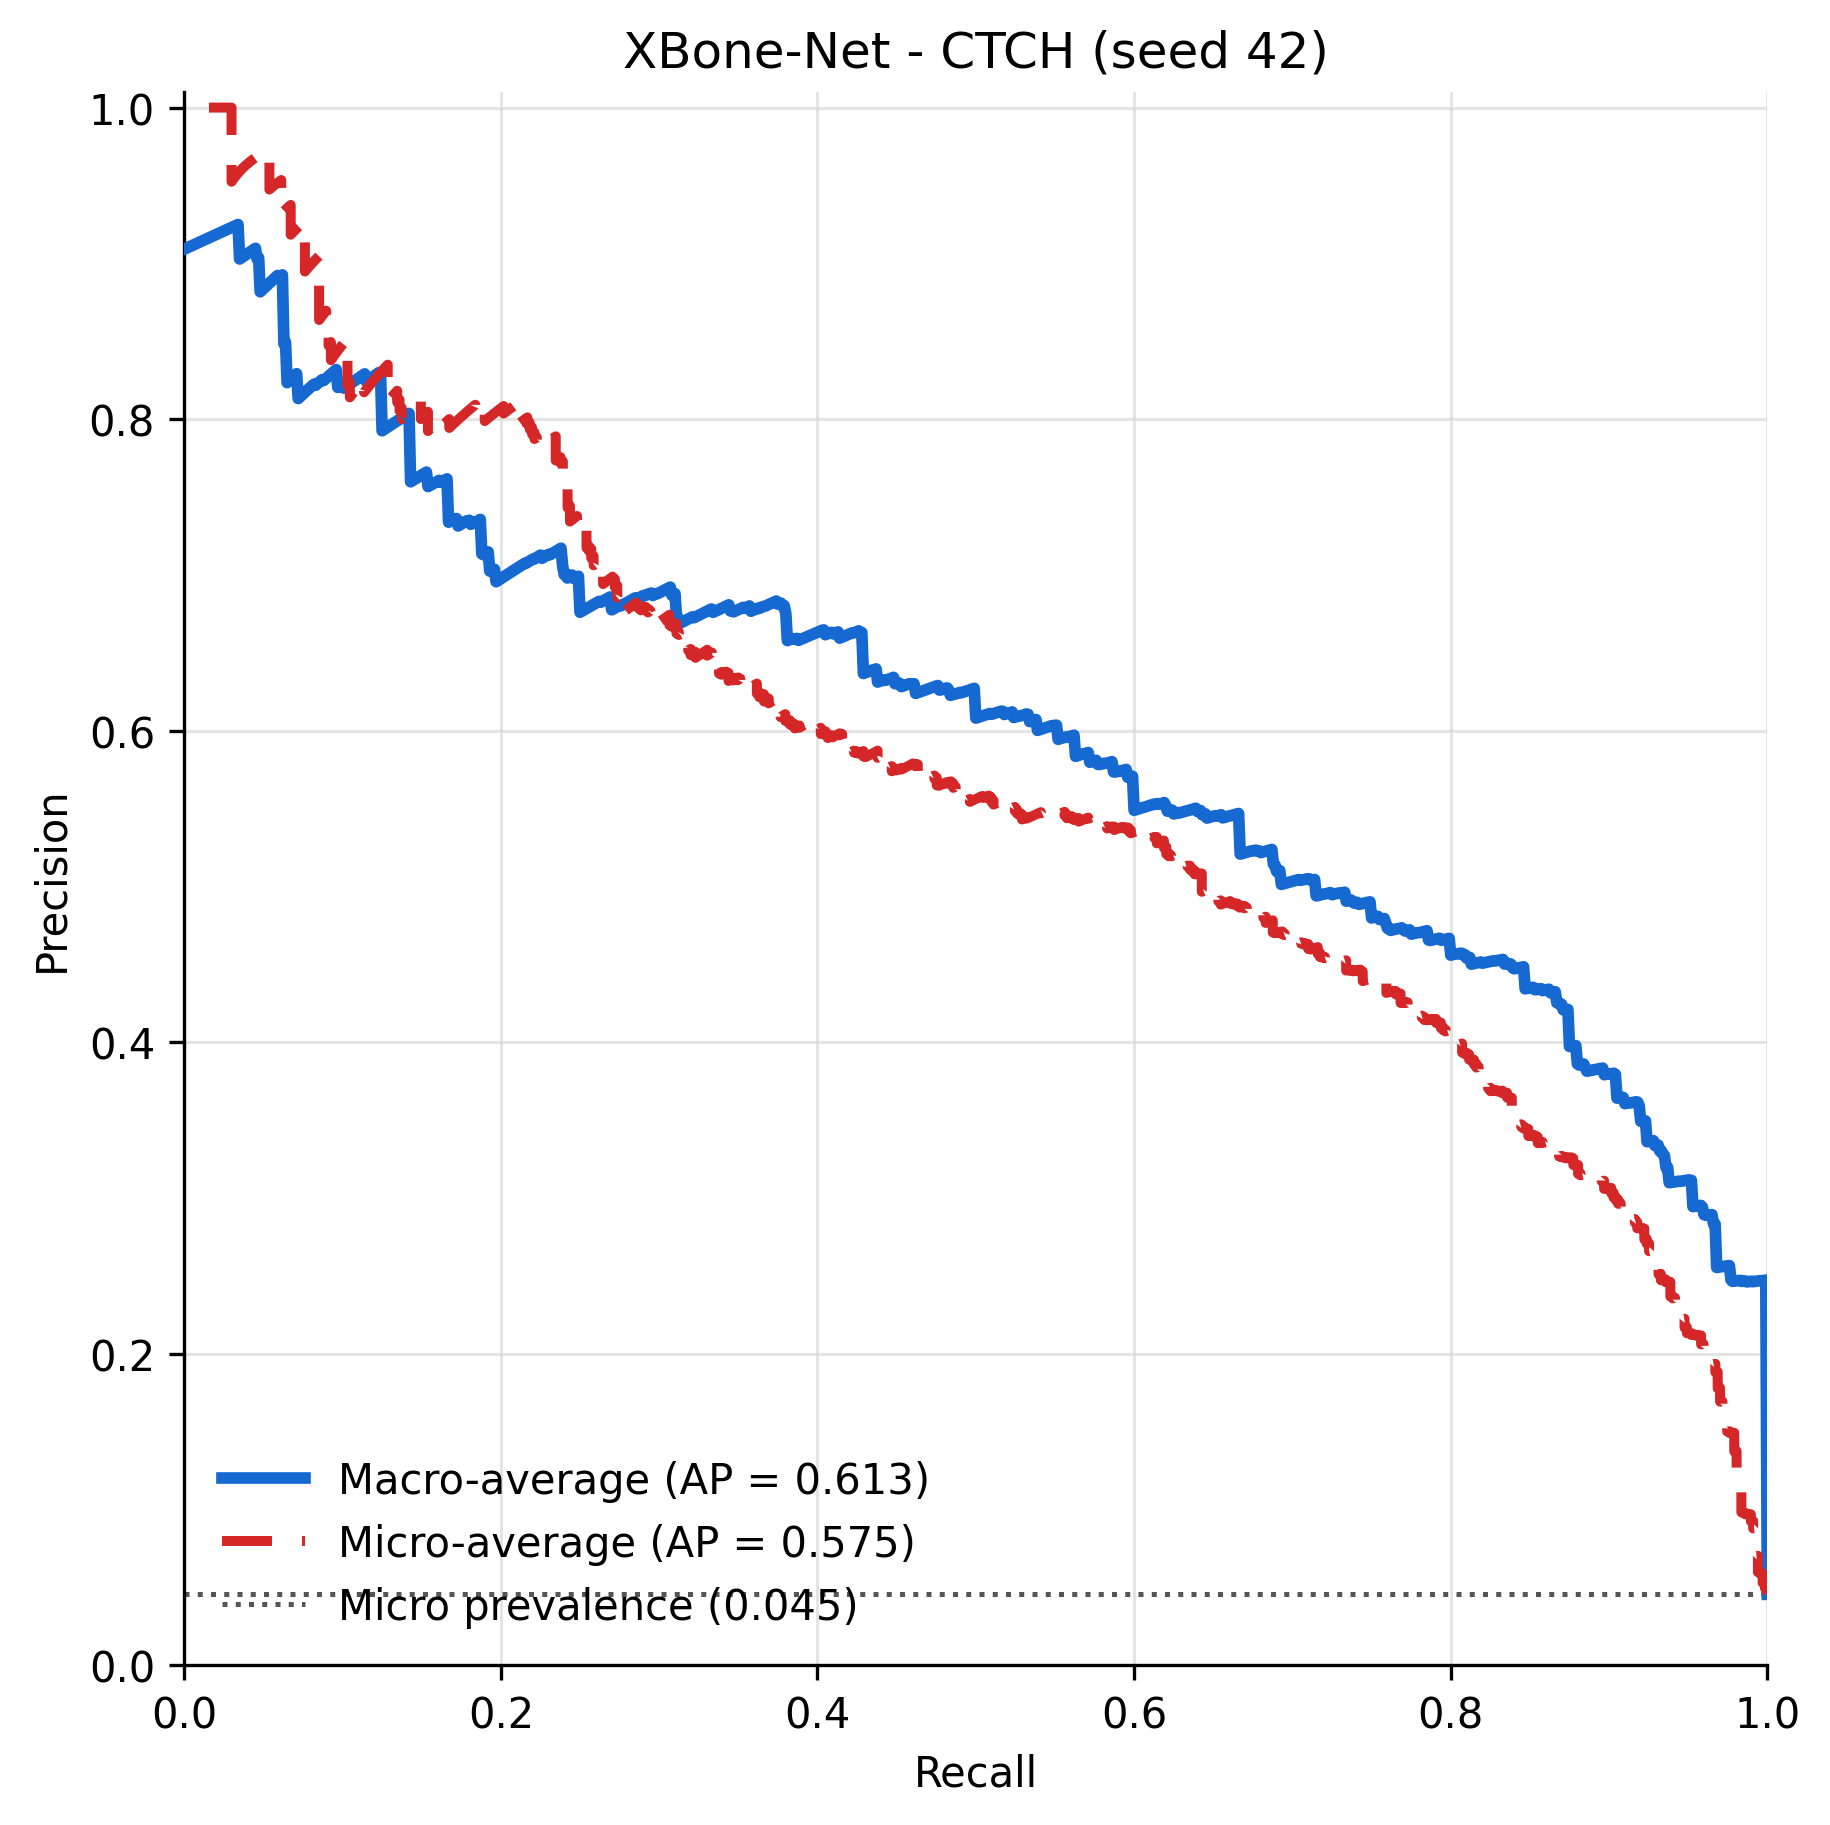
\includegraphics[width=\textwidth]{images/chapter4_draft/appendix/pr_ctch_seed42.png}
\caption{Precision--Recall trên CTCH, seed 42}
\end{subfigure}
\caption{Đường cong xếp hạng xác suất của XBone-Net trên CTCH}
\label{fig:app_ch4_ctch_curves}
\end{figure}

\begin{figure}[H]
\centering
\begin{subfigure}[t]{0.49\textwidth}
\centering
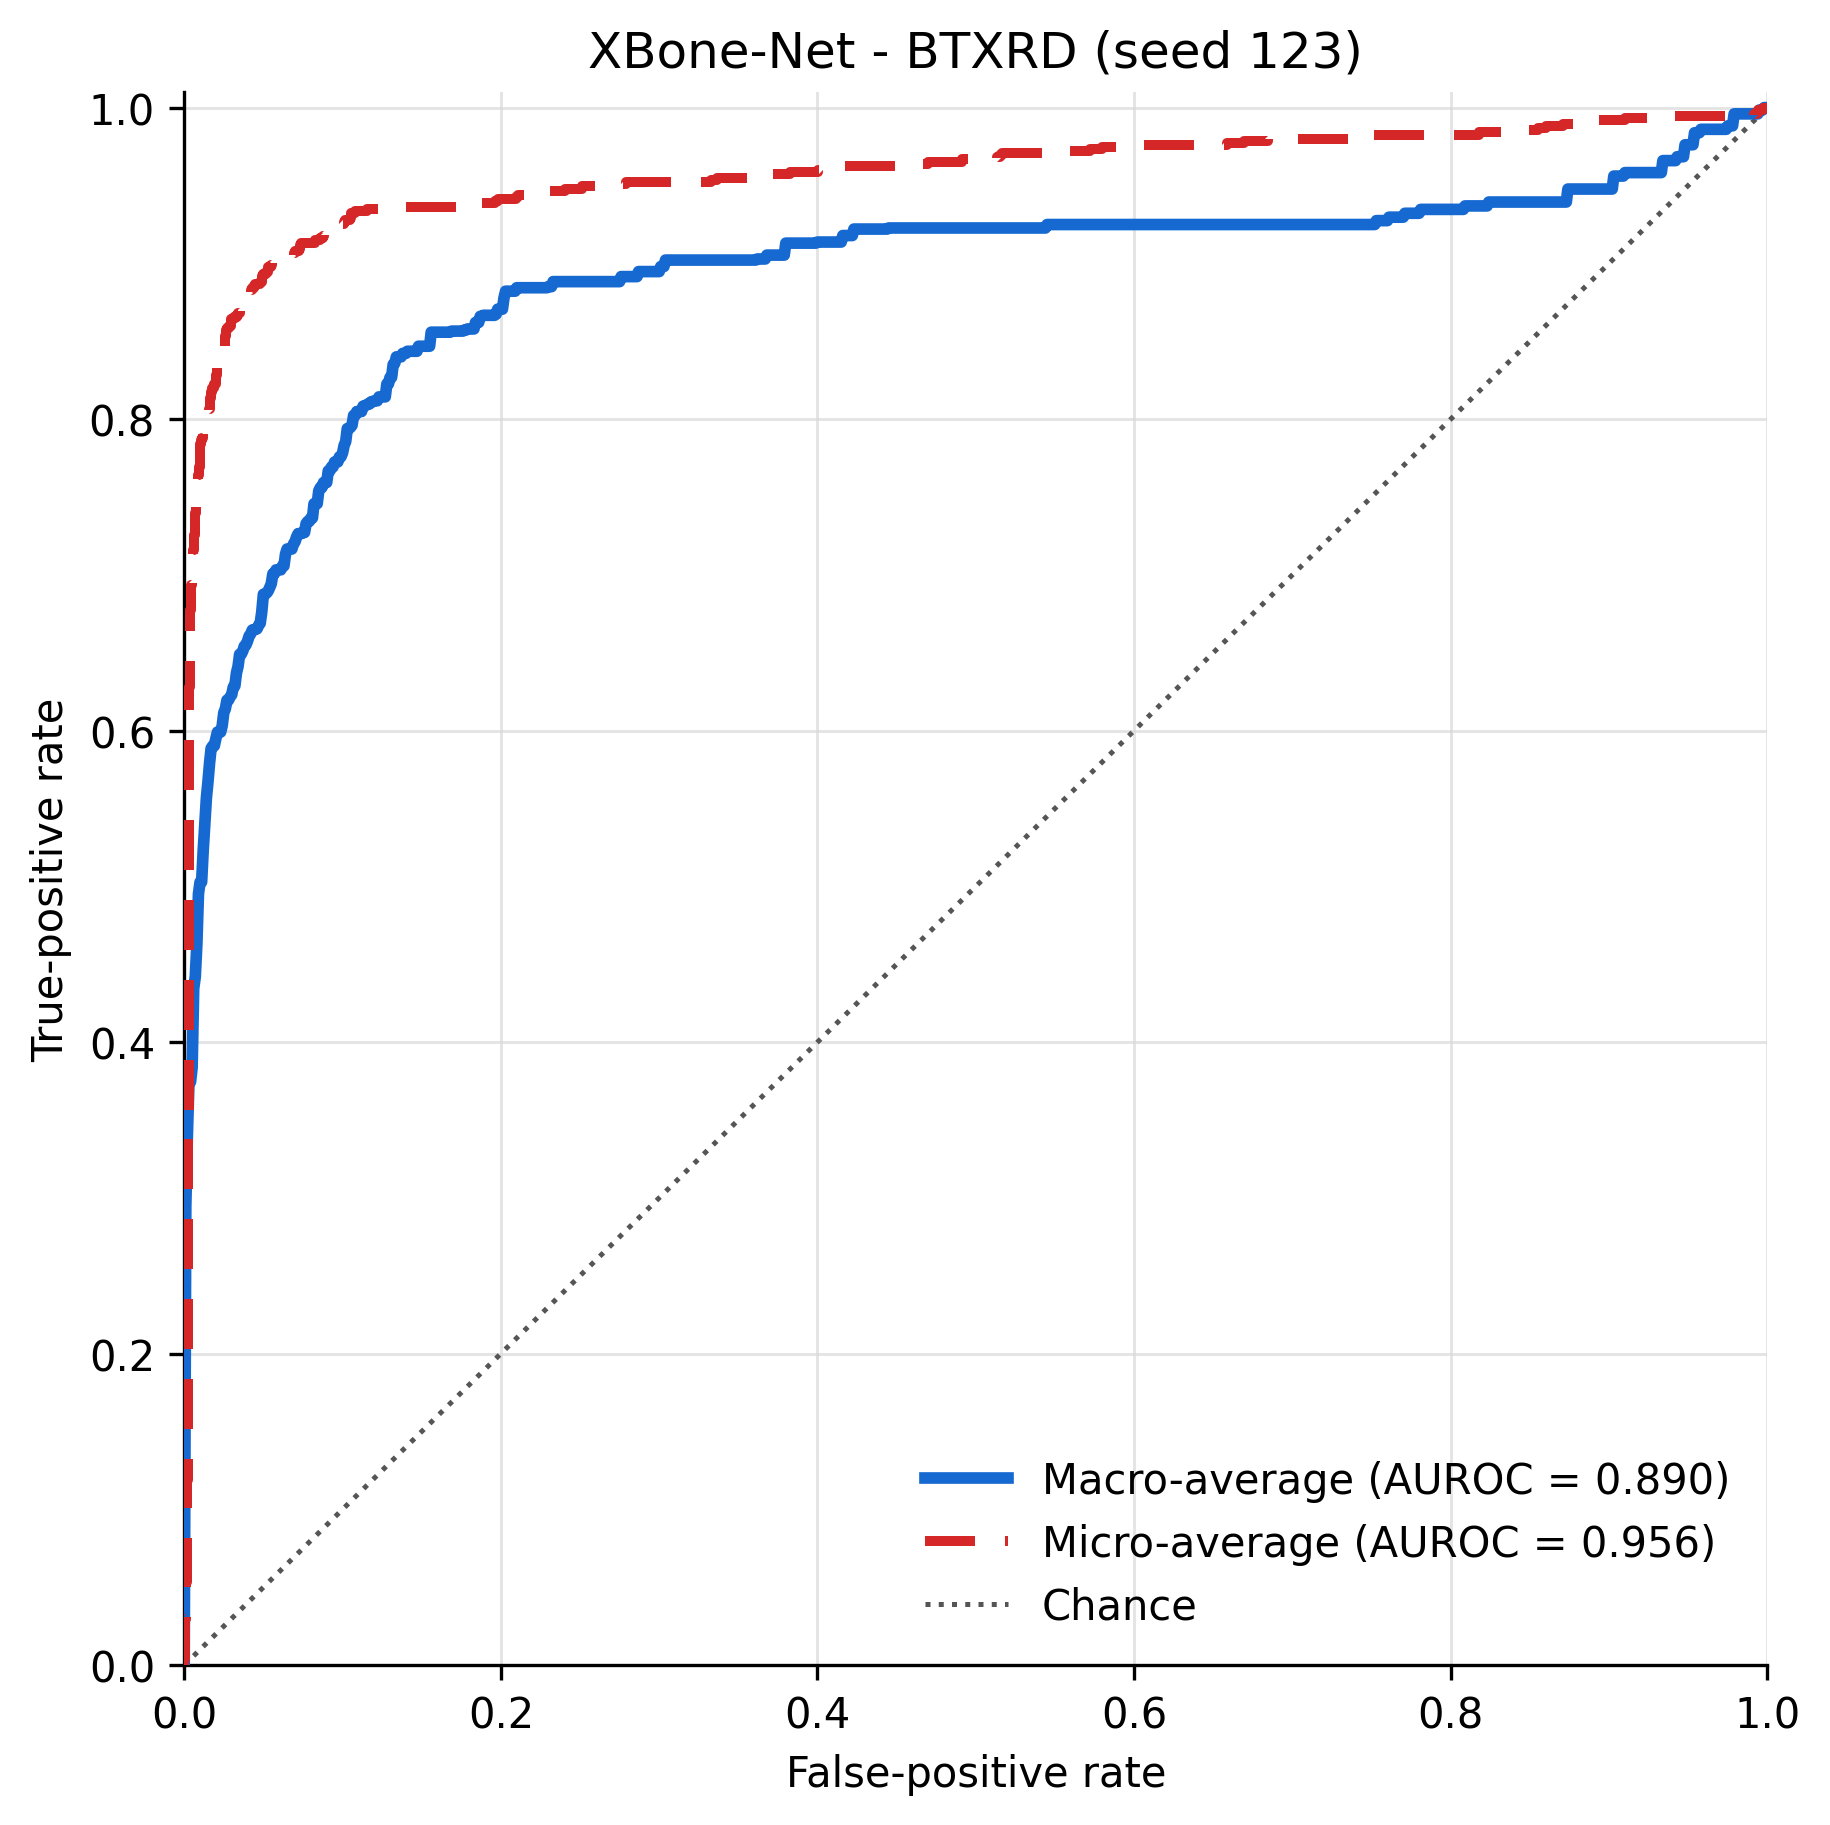
\includegraphics[width=\textwidth]{images/chapter4_draft/appendix/roc_btxrd_seed123.png}
\caption{ROC trên BTXRD, seed 123}
\end{subfigure}
\hfill
\begin{subfigure}[t]{0.49\textwidth}
\centering
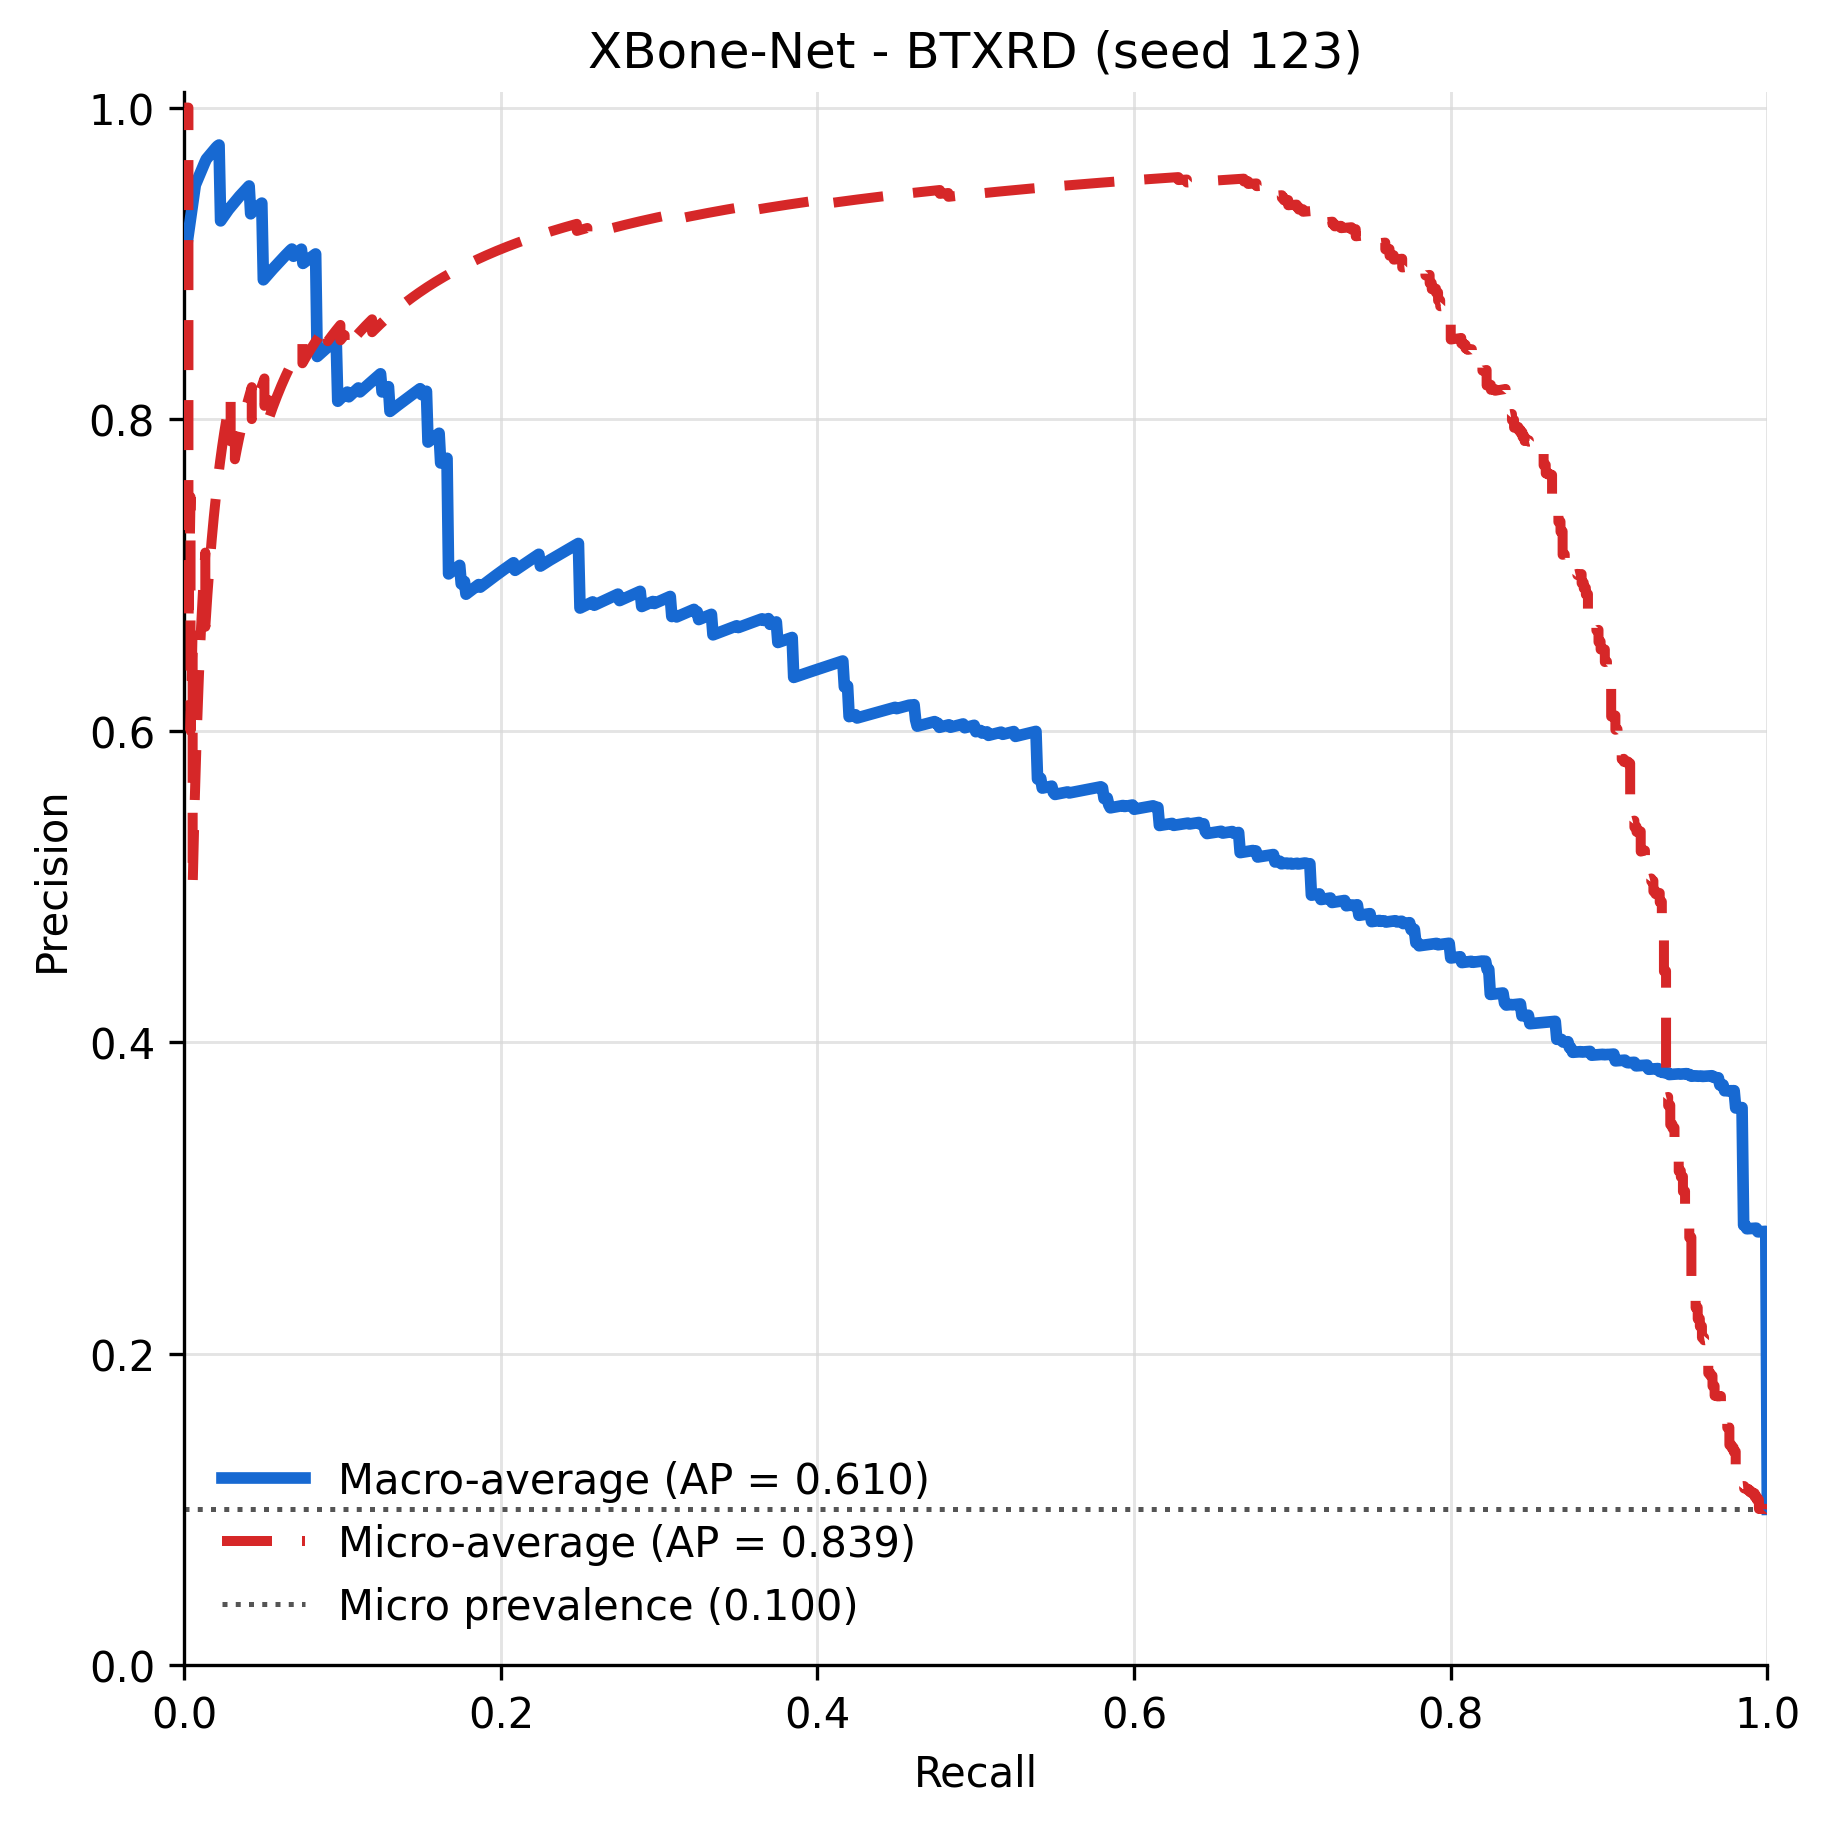
\includegraphics[width=\textwidth]{images/chapter4_draft/appendix/pr_btxrd_seed123.png}
\caption{Precision--Recall trên BTXRD, seed 123}
\end{subfigure}
\caption{Đường cong xếp hạng xác suất của XBone-Net trên BTXRD}
\label{fig:app_ch4_btxrd_curves}
\end{figure}

\begin{figure}[H]
\centering
\begin{subfigure}[t]{0.49\textwidth}
\centering
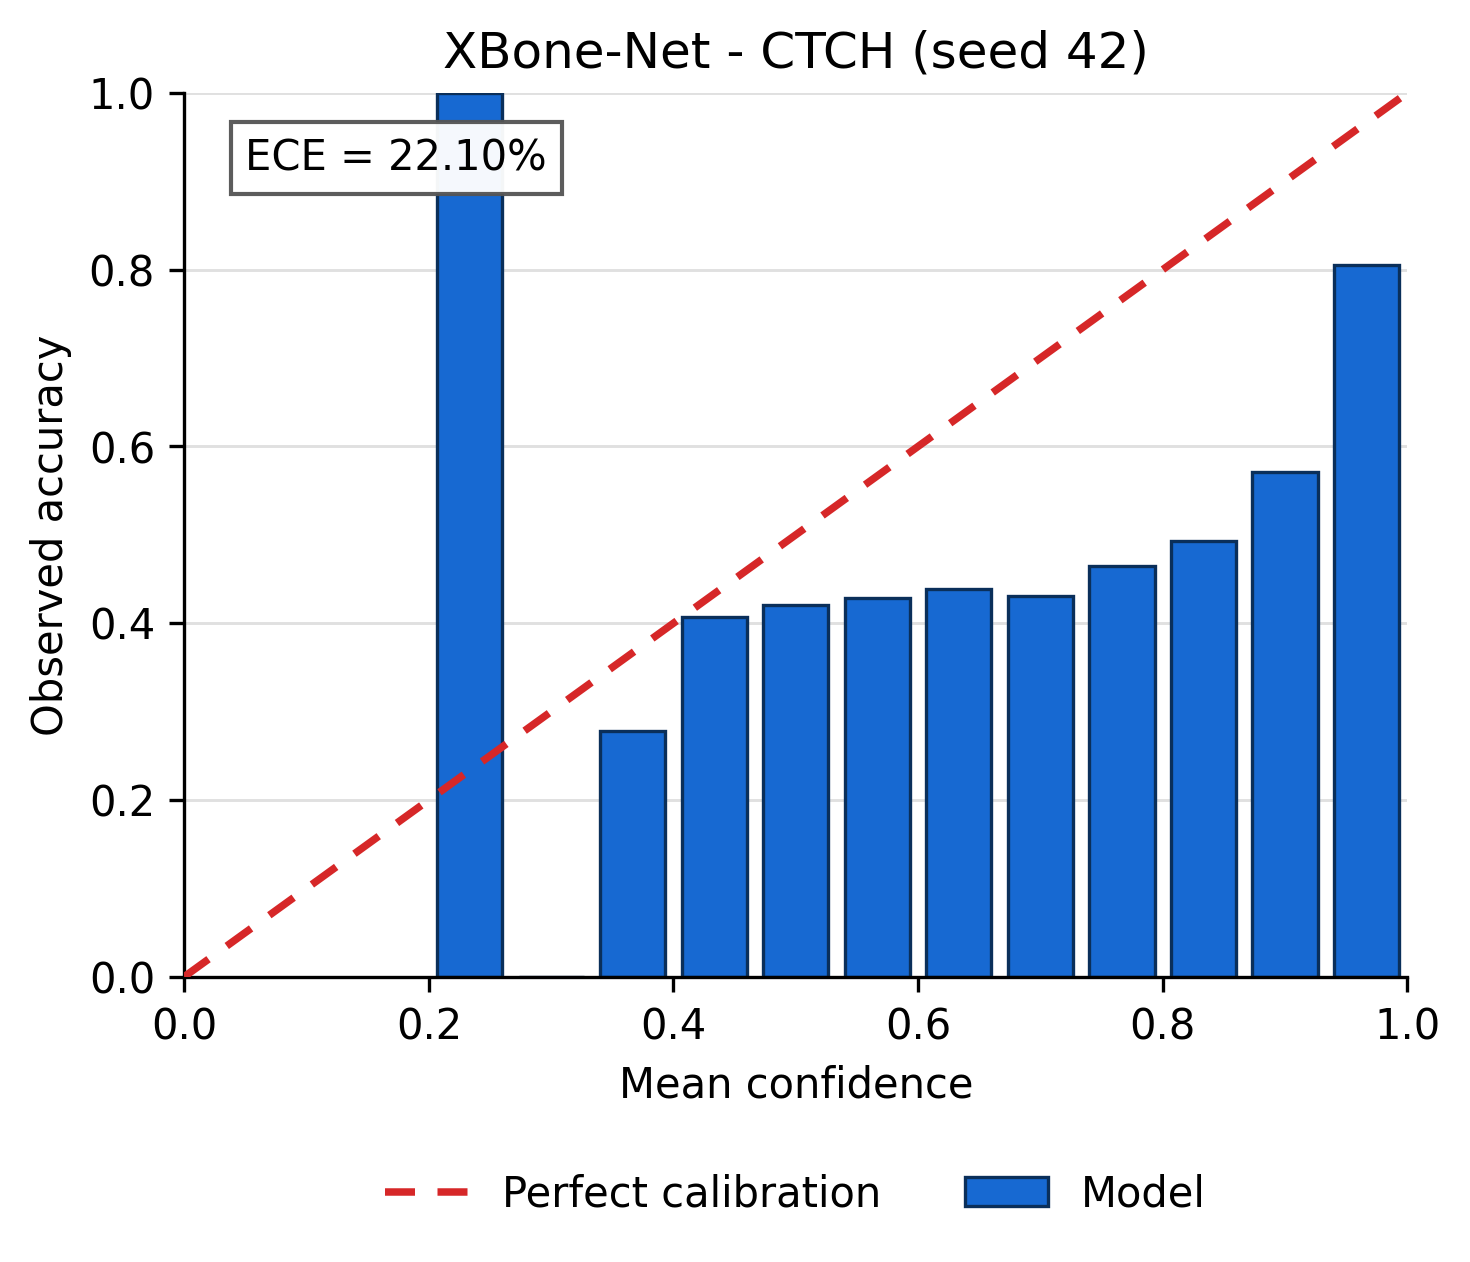
\includegraphics[width=\textwidth]{images/chapter4_draft/appendix/calibration_ctch_seed42.png}
\caption{CTCH, seed 42}
\end{subfigure}
\hfill
\begin{subfigure}[t]{0.49\textwidth}
\centering
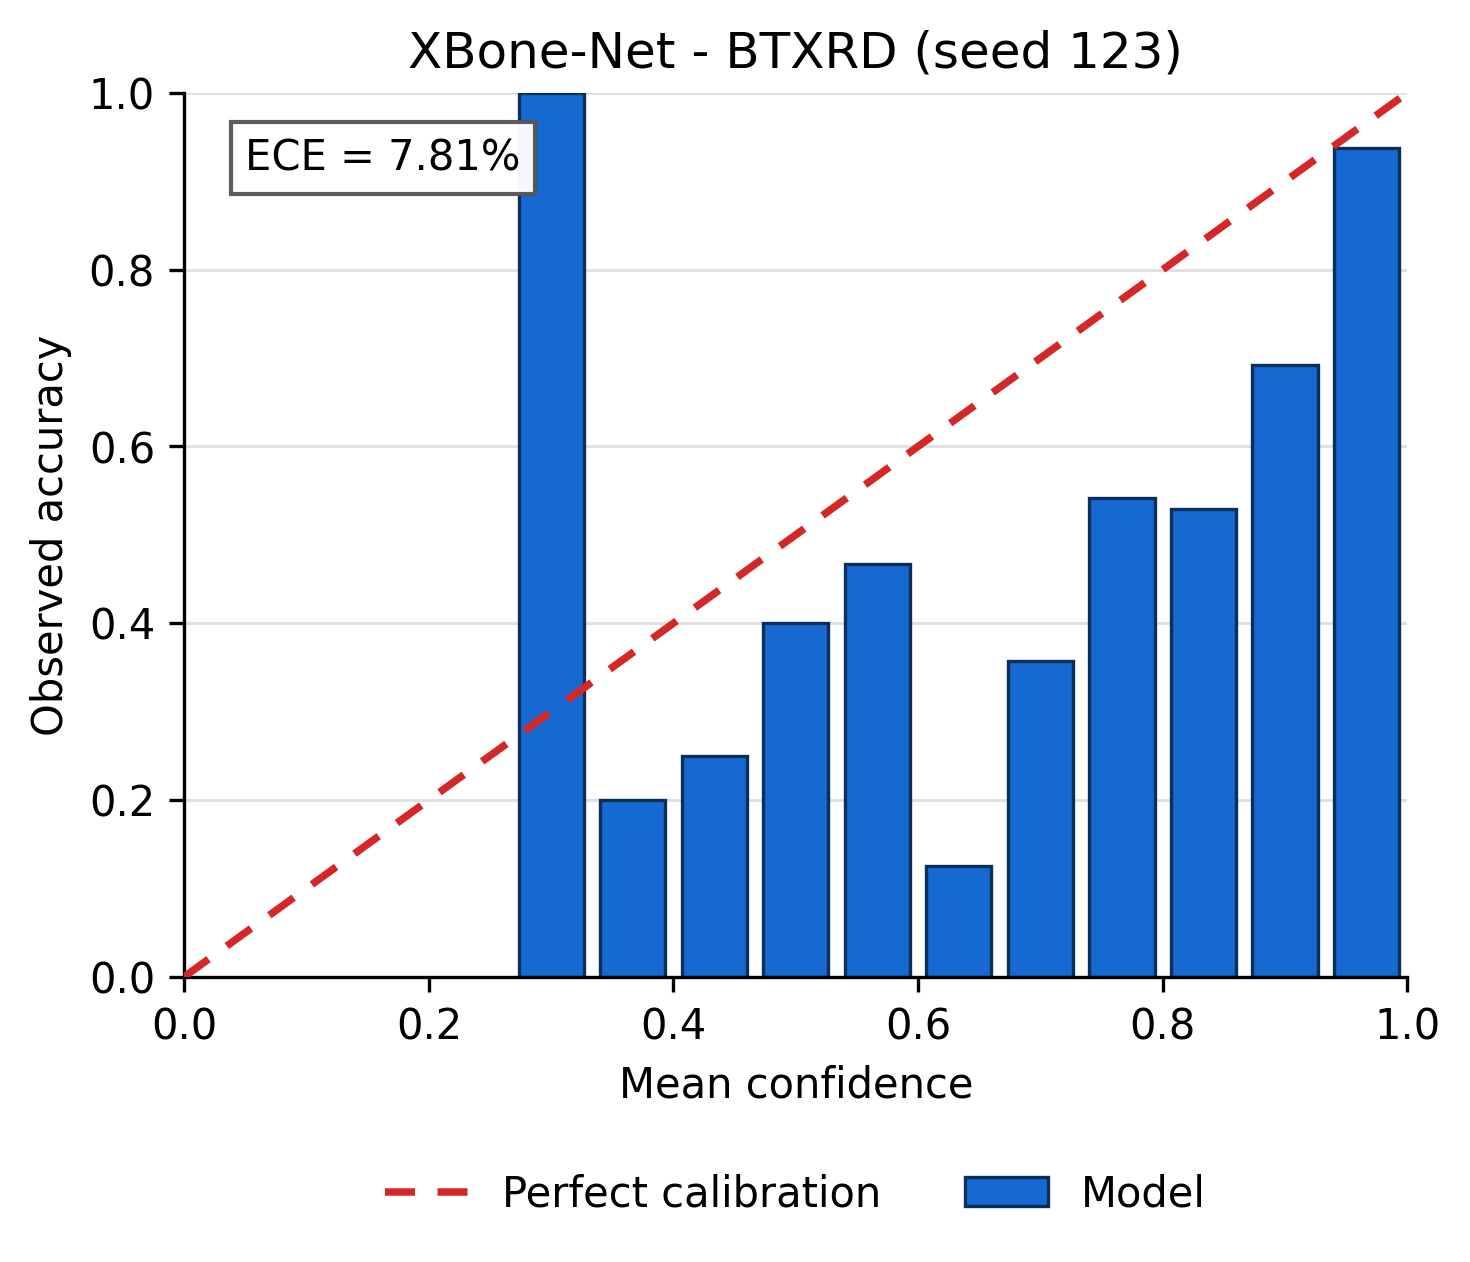
\includegraphics[width=\textwidth]{images/chapter4_draft/appendix/calibration_btxrd_seed123.png}
\caption{BTXRD, seed 123}
\end{subfigure}
\caption{Reliability diagram của XBone-Net; đường chéo biểu thị hiệu chuẩn lý tưởng}
\label{fig:app_ch4_calibration}
\end{figure}

Reliability diagram cho thấy ECE của hai lần chạy khác nhau đáng kể giữa CTCH và BTXRD. Do các hình được chọn ở hai hạt giống khác nhau và chưa biểu diễn độ biến thiên giữa seed, kết luận về hiệu chuẩn phải dựa trên bảng tổng hợp ba hạt giống trong bản báo cáo chính; các hình này chỉ hỗ trợ quan sát vùng xác suất bị over-confidence hoặc under-confidence.

\section{Tổng quan đối sánh phân loại}

\begin{figure}[H]
\centering
\begin{subfigure}[t]{0.49\textwidth}
\centering
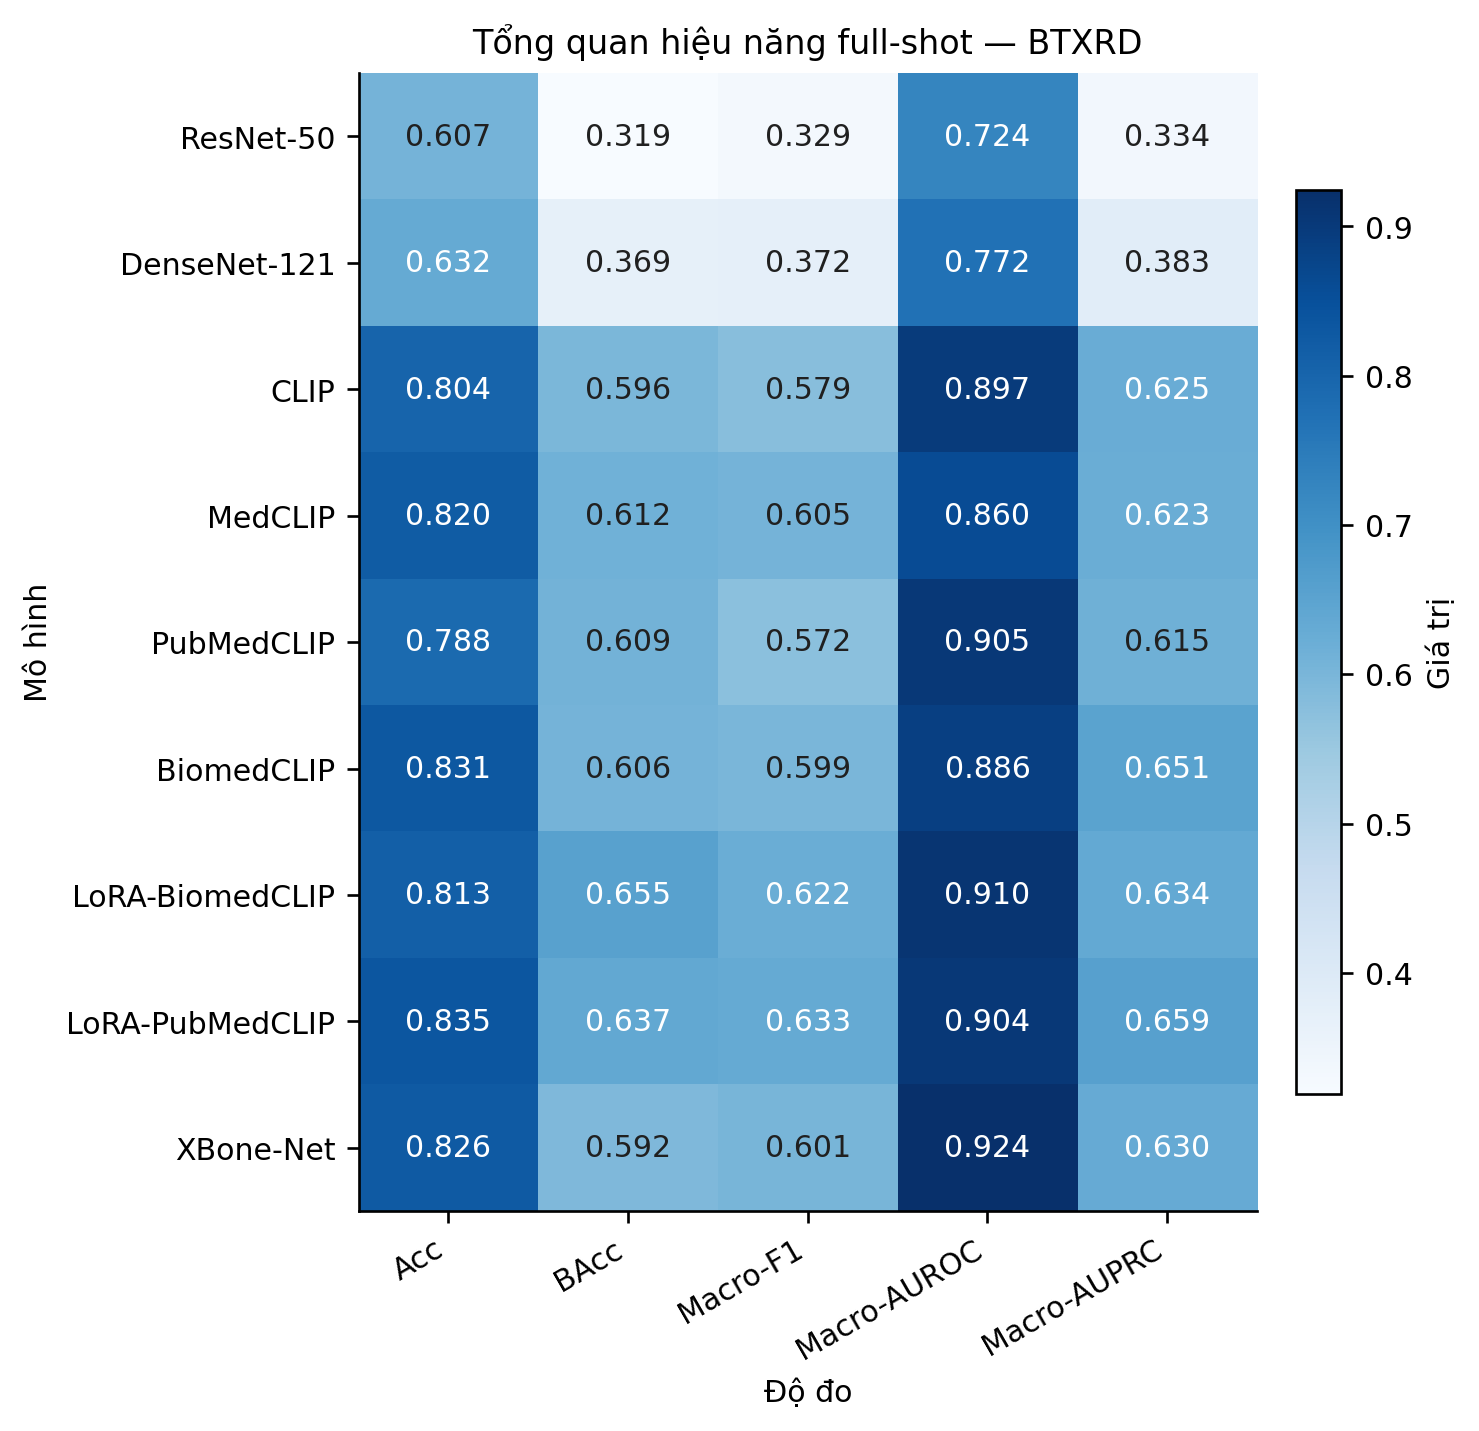
\includegraphics[width=\textwidth]{images/chapter4_draft/appendix/fullshot_btxrd_heatmap.png}
\caption{BTXRD}
\end{subfigure}
\hfill
\begin{subfigure}[t]{0.49\textwidth}
\centering
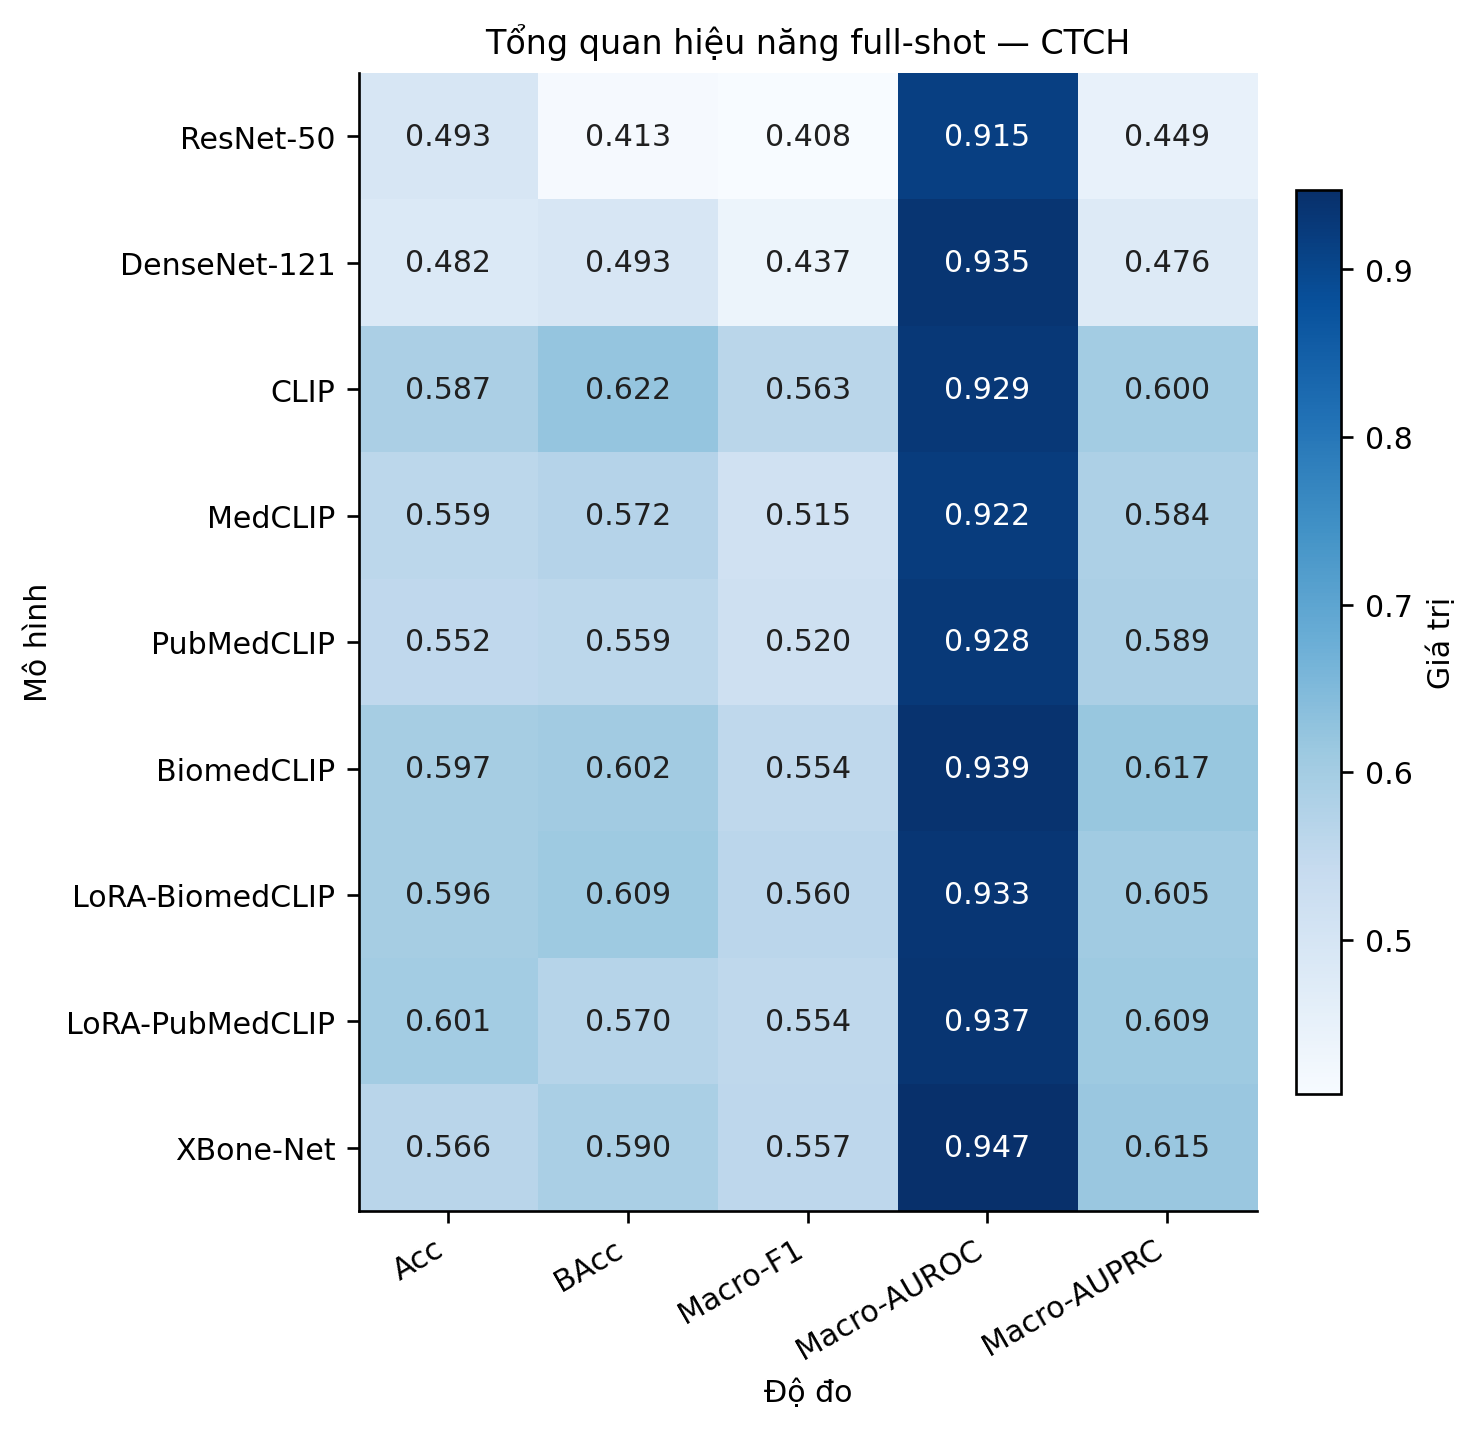
\includegraphics[width=\textwidth]{images/chapter4_draft/appendix/fullshot_ctch_heatmap.png}
\caption{CTCH}
\end{subfigure}
\caption{Heatmap tổng hợp năm độ đo của các mô hình trong thiết lập full-shot}
\label{fig:app_ch4_fullshot_heatmaps}
\end{figure}

\begin{figure}[H]
\centering
\begin{subfigure}[t]{0.49\textwidth}
\centering
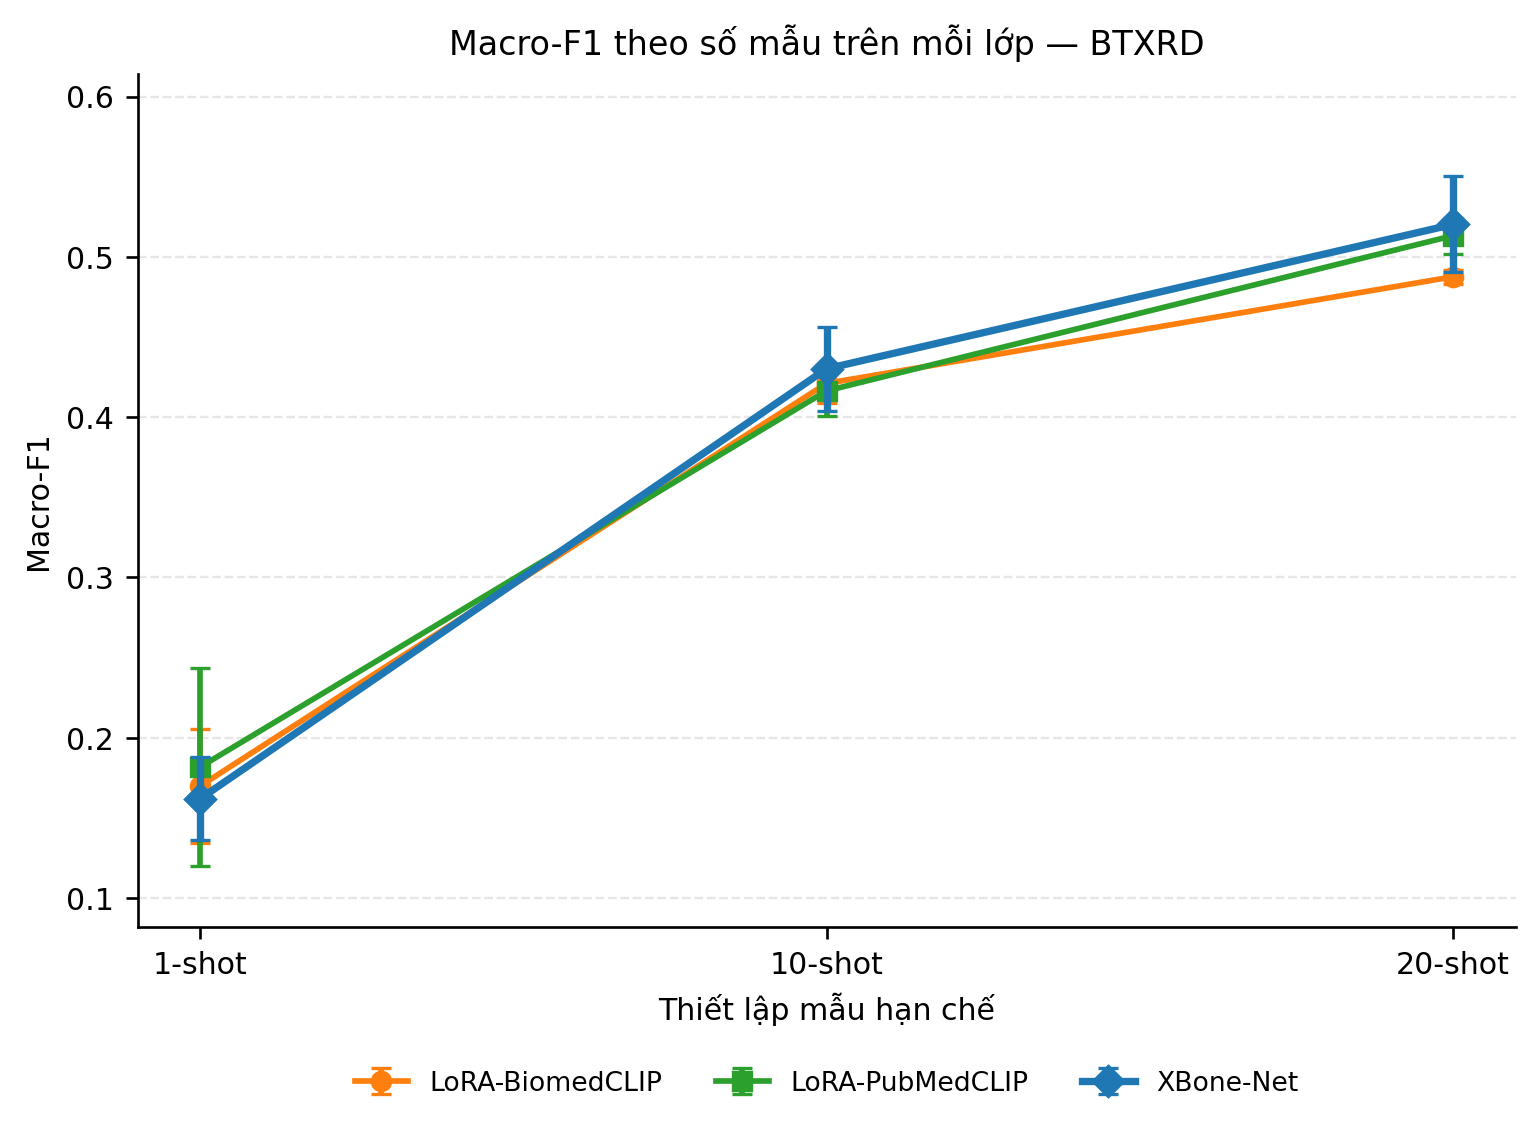
\includegraphics[width=\textwidth]{images/chapter4_draft/appendix/fewshot_btxrd_line.png}
\caption{BTXRD}
\end{subfigure}
\hfill
\begin{subfigure}[t]{0.49\textwidth}
\centering
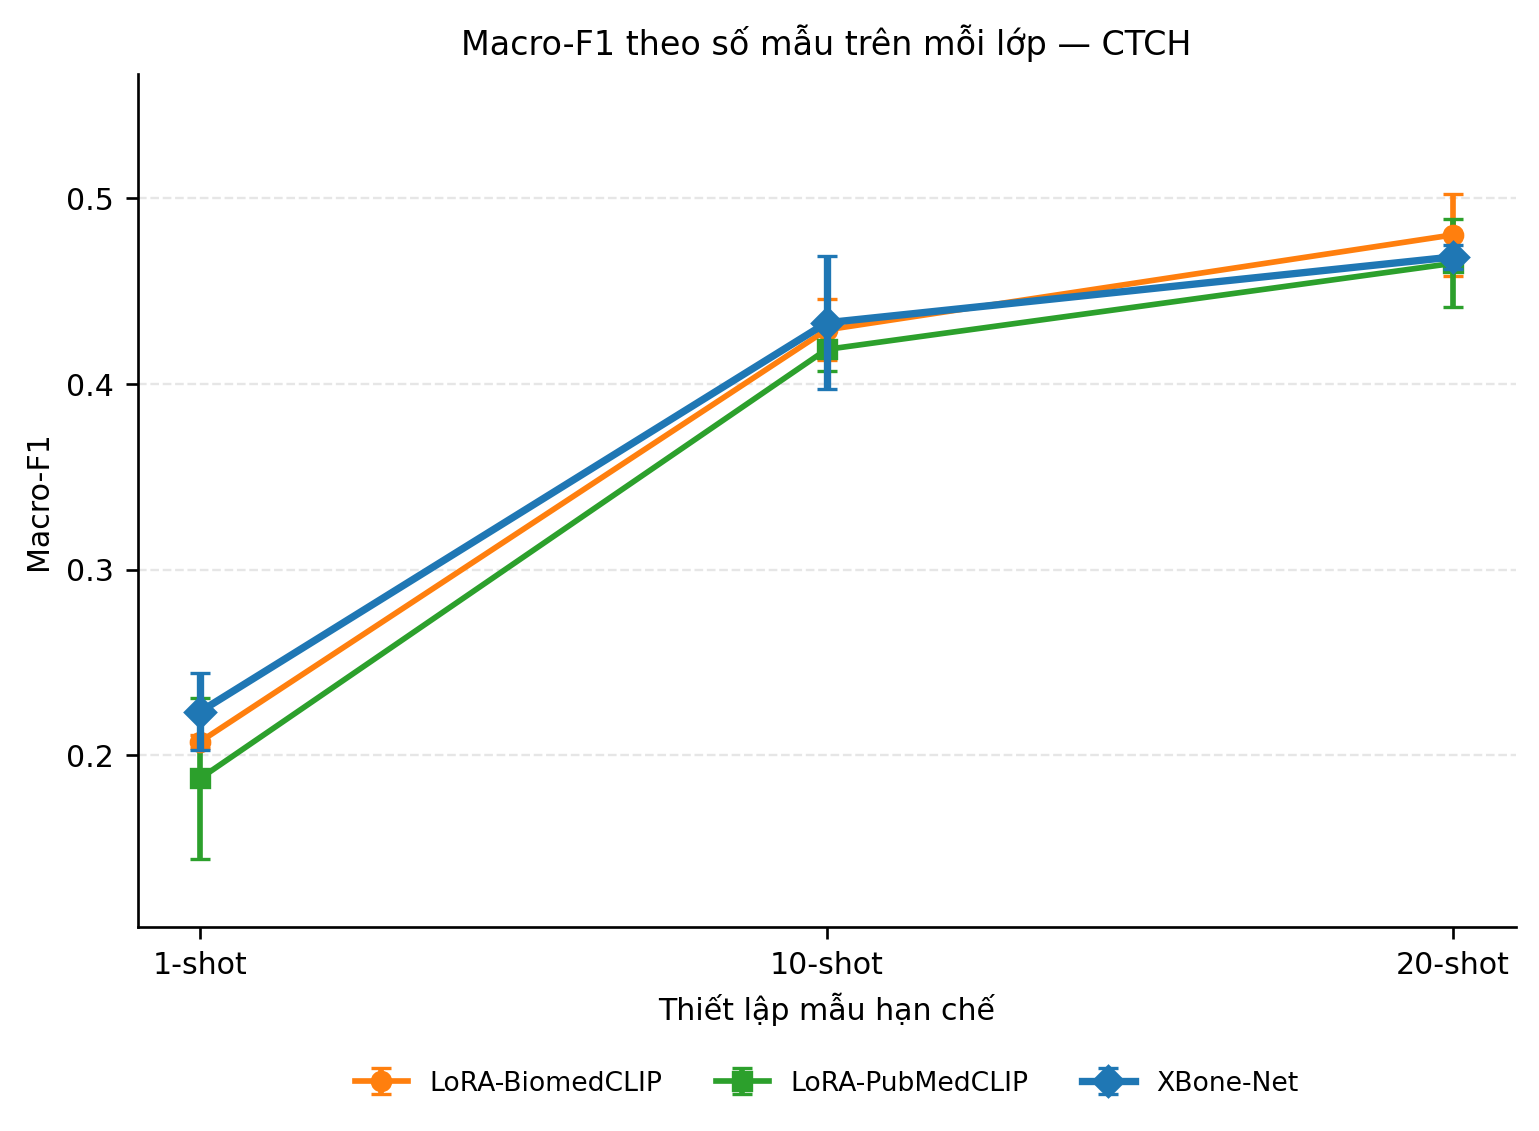
\includegraphics[width=\textwidth]{images/chapter4_draft/appendix/fewshot_ctch_line.png}
\caption{CTCH}
\end{subfigure}
\caption{Đường biến thiên Macro-F1 theo số mẫu huấn luyện trên mỗi lớp}
\label{fig:app_ch4_fewshot_lines}
\end{figure}

\begin{figure}[H]
\centering
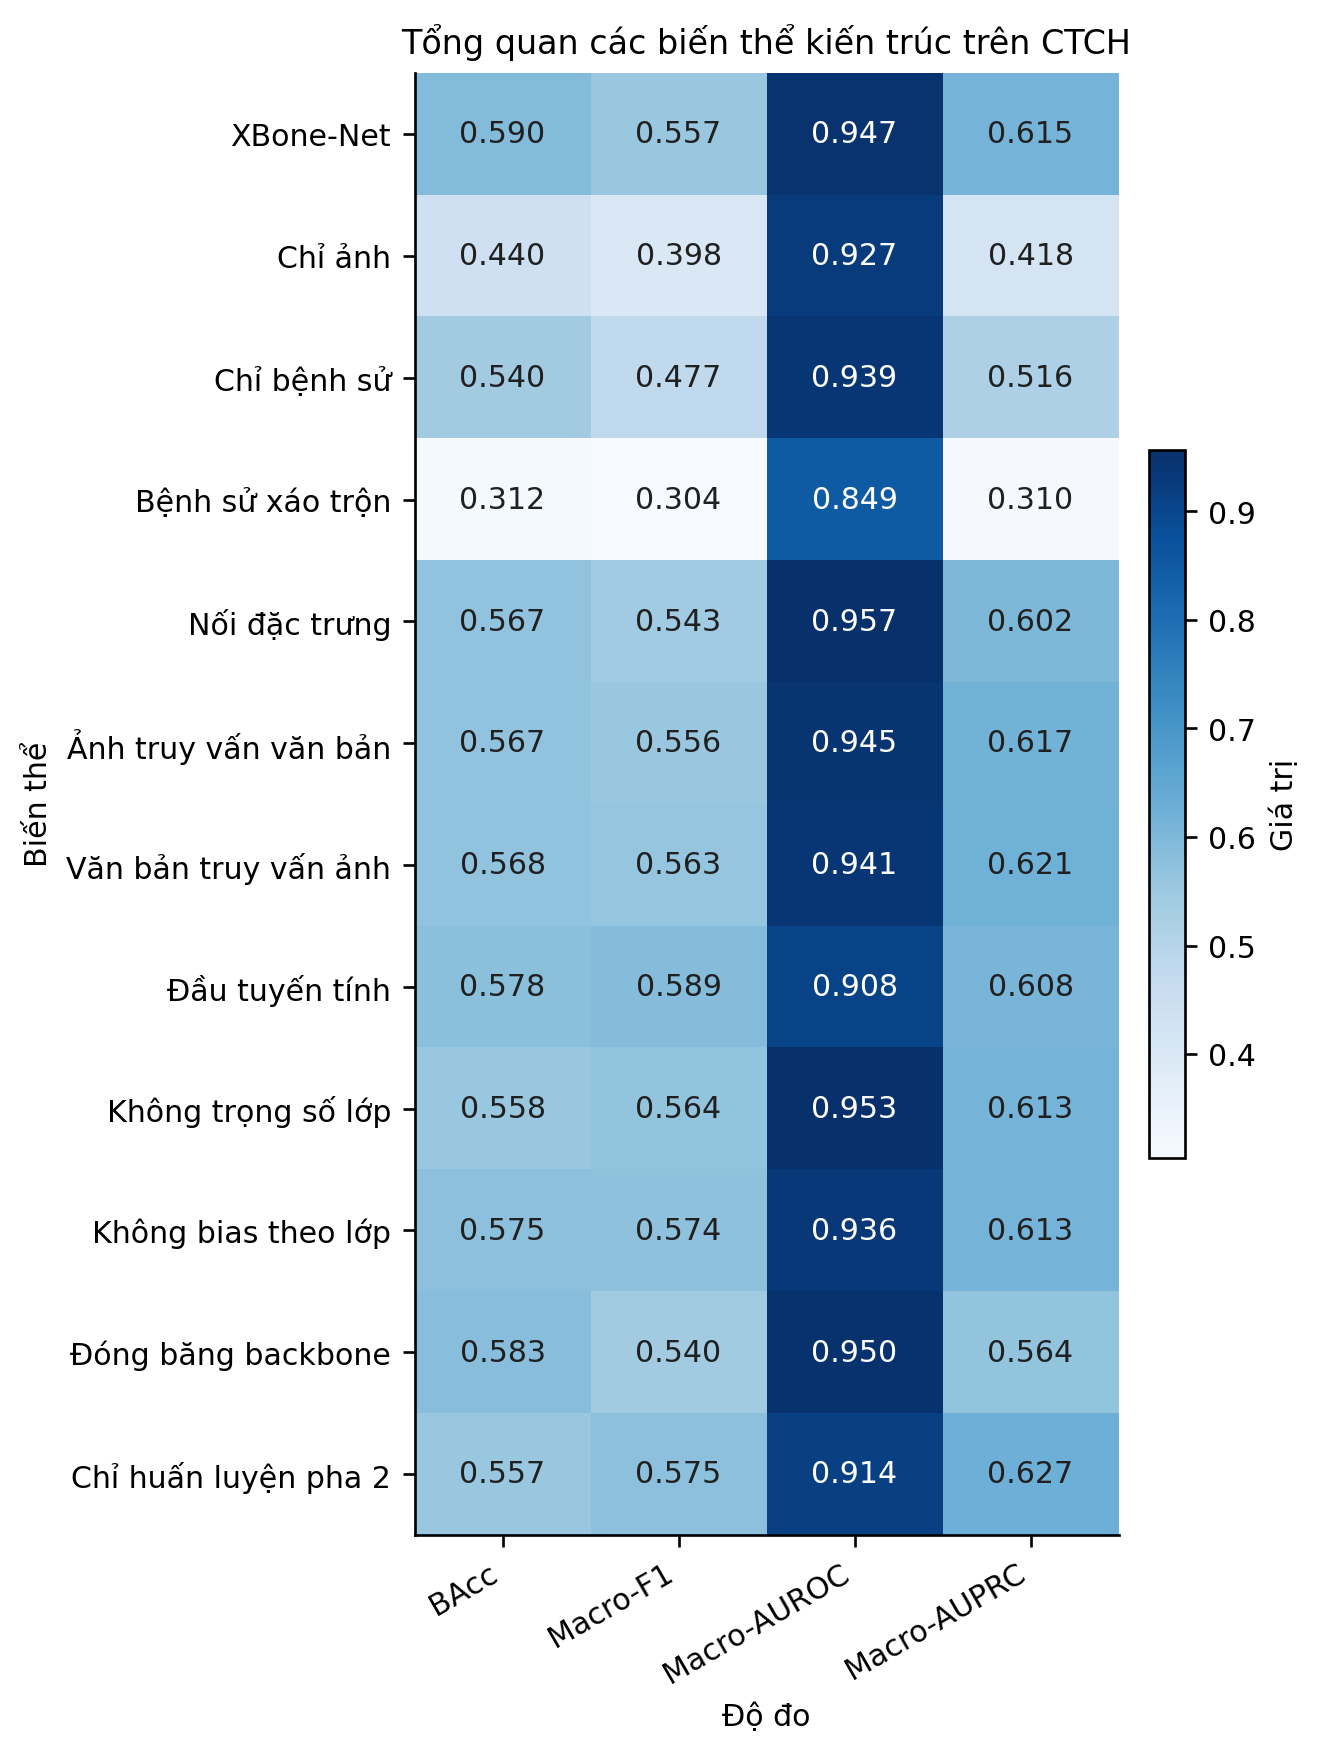
\includegraphics[width=0.86\textwidth]{images/chapter4_draft/appendix/ablation_metric_heatmap.png}
\caption{Heatmap đối sánh đồng thời BAcc, Macro-F1, Macro-AUROC và Macro-AUPRC của các biến thể trên CTCH}
\label{fig:app_ch4_ablation_heatmap}
\end{figure}

Hai heatmap full-shot giúp quan sát sự thay đổi thứ hạng theo độ đo thay vì chỉ theo một chỉ số tổng hợp. Các đường few-shot biểu diễn xu hướng và độ biến thiên giữa hạt giống, trong khi heatmap ablation cho thấy một biến thể có thể cải thiện Macro-F1 nhưng đồng thời làm giảm Macro-AUROC. Các hình này được đặt ở phụ lục để hỗ trợ tra cứu, còn phần chính giữ các đồ thị trực tiếp phục vụ lập luận.

\section{Phân phối OOD score}

\begin{figure}[H]
\centering
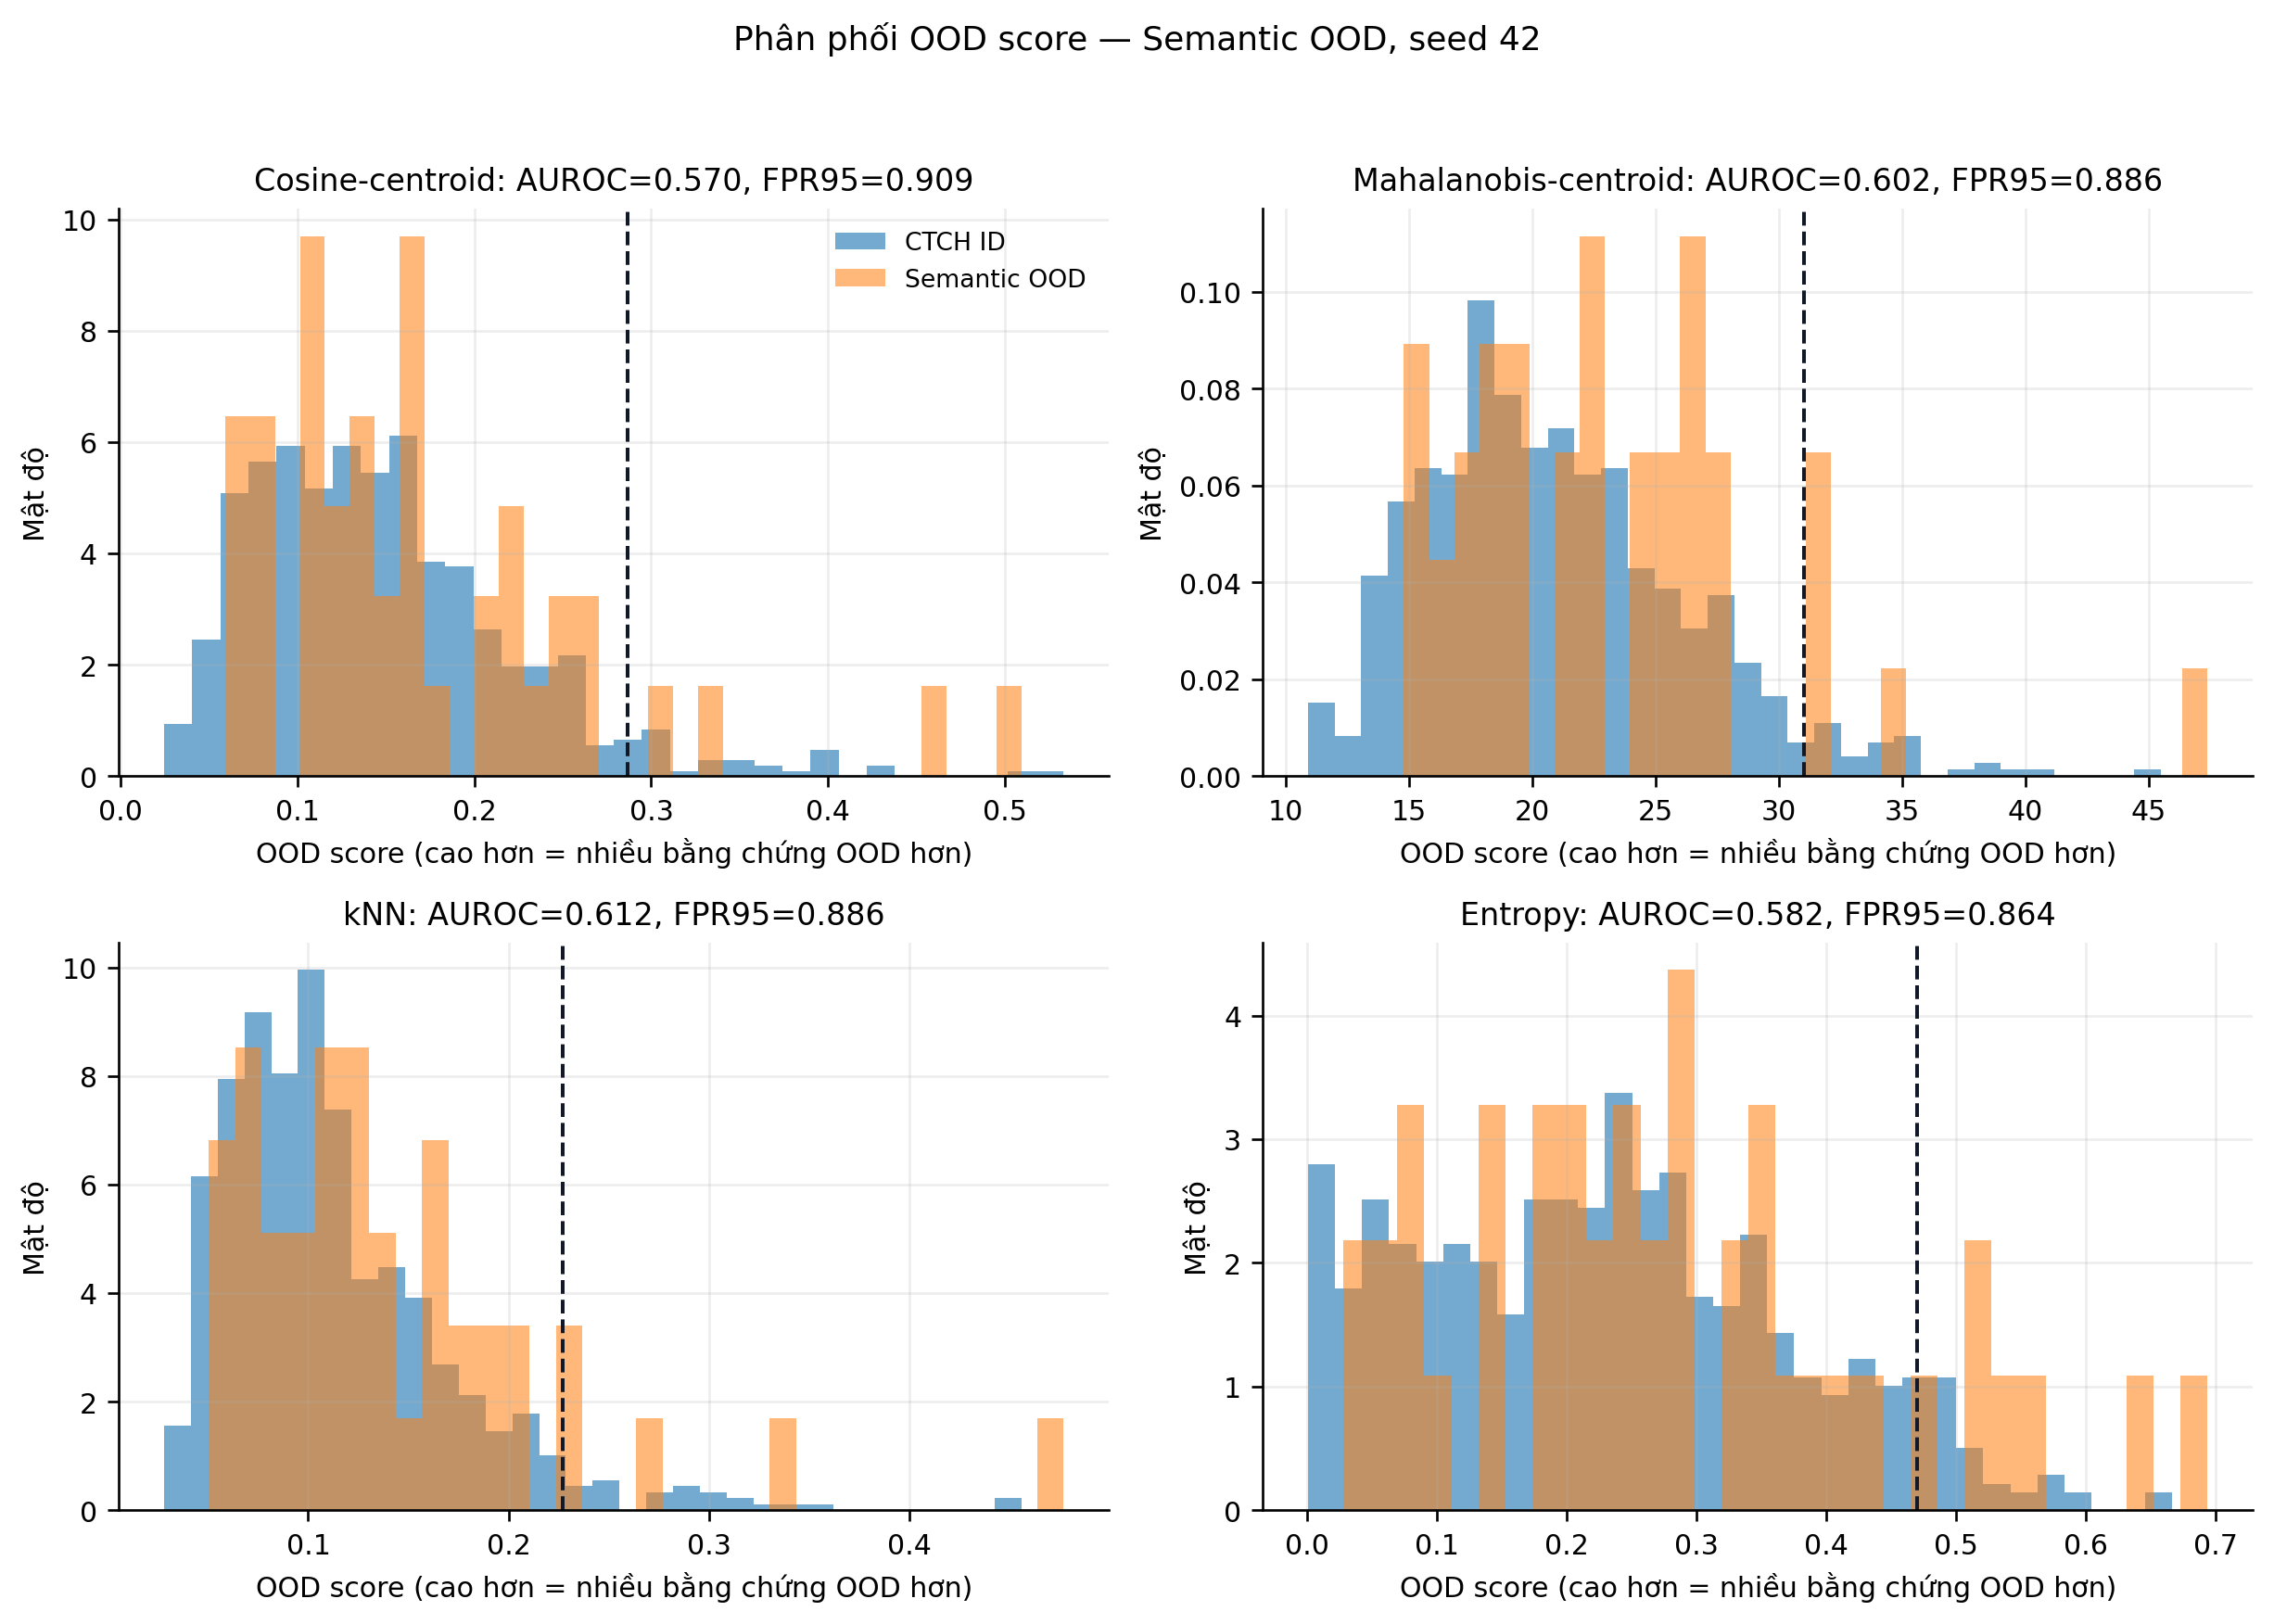
\includegraphics[width=\textwidth]{images/chapter4_draft/appendix/ood_distribution_semantic_ood.png}
\caption{Phân phối score của semantic OOD và CTCH-ID tại seed 42}
\label{fig:app_ch4_ood_semantic}
\end{figure}

\begin{figure}[H]
\centering
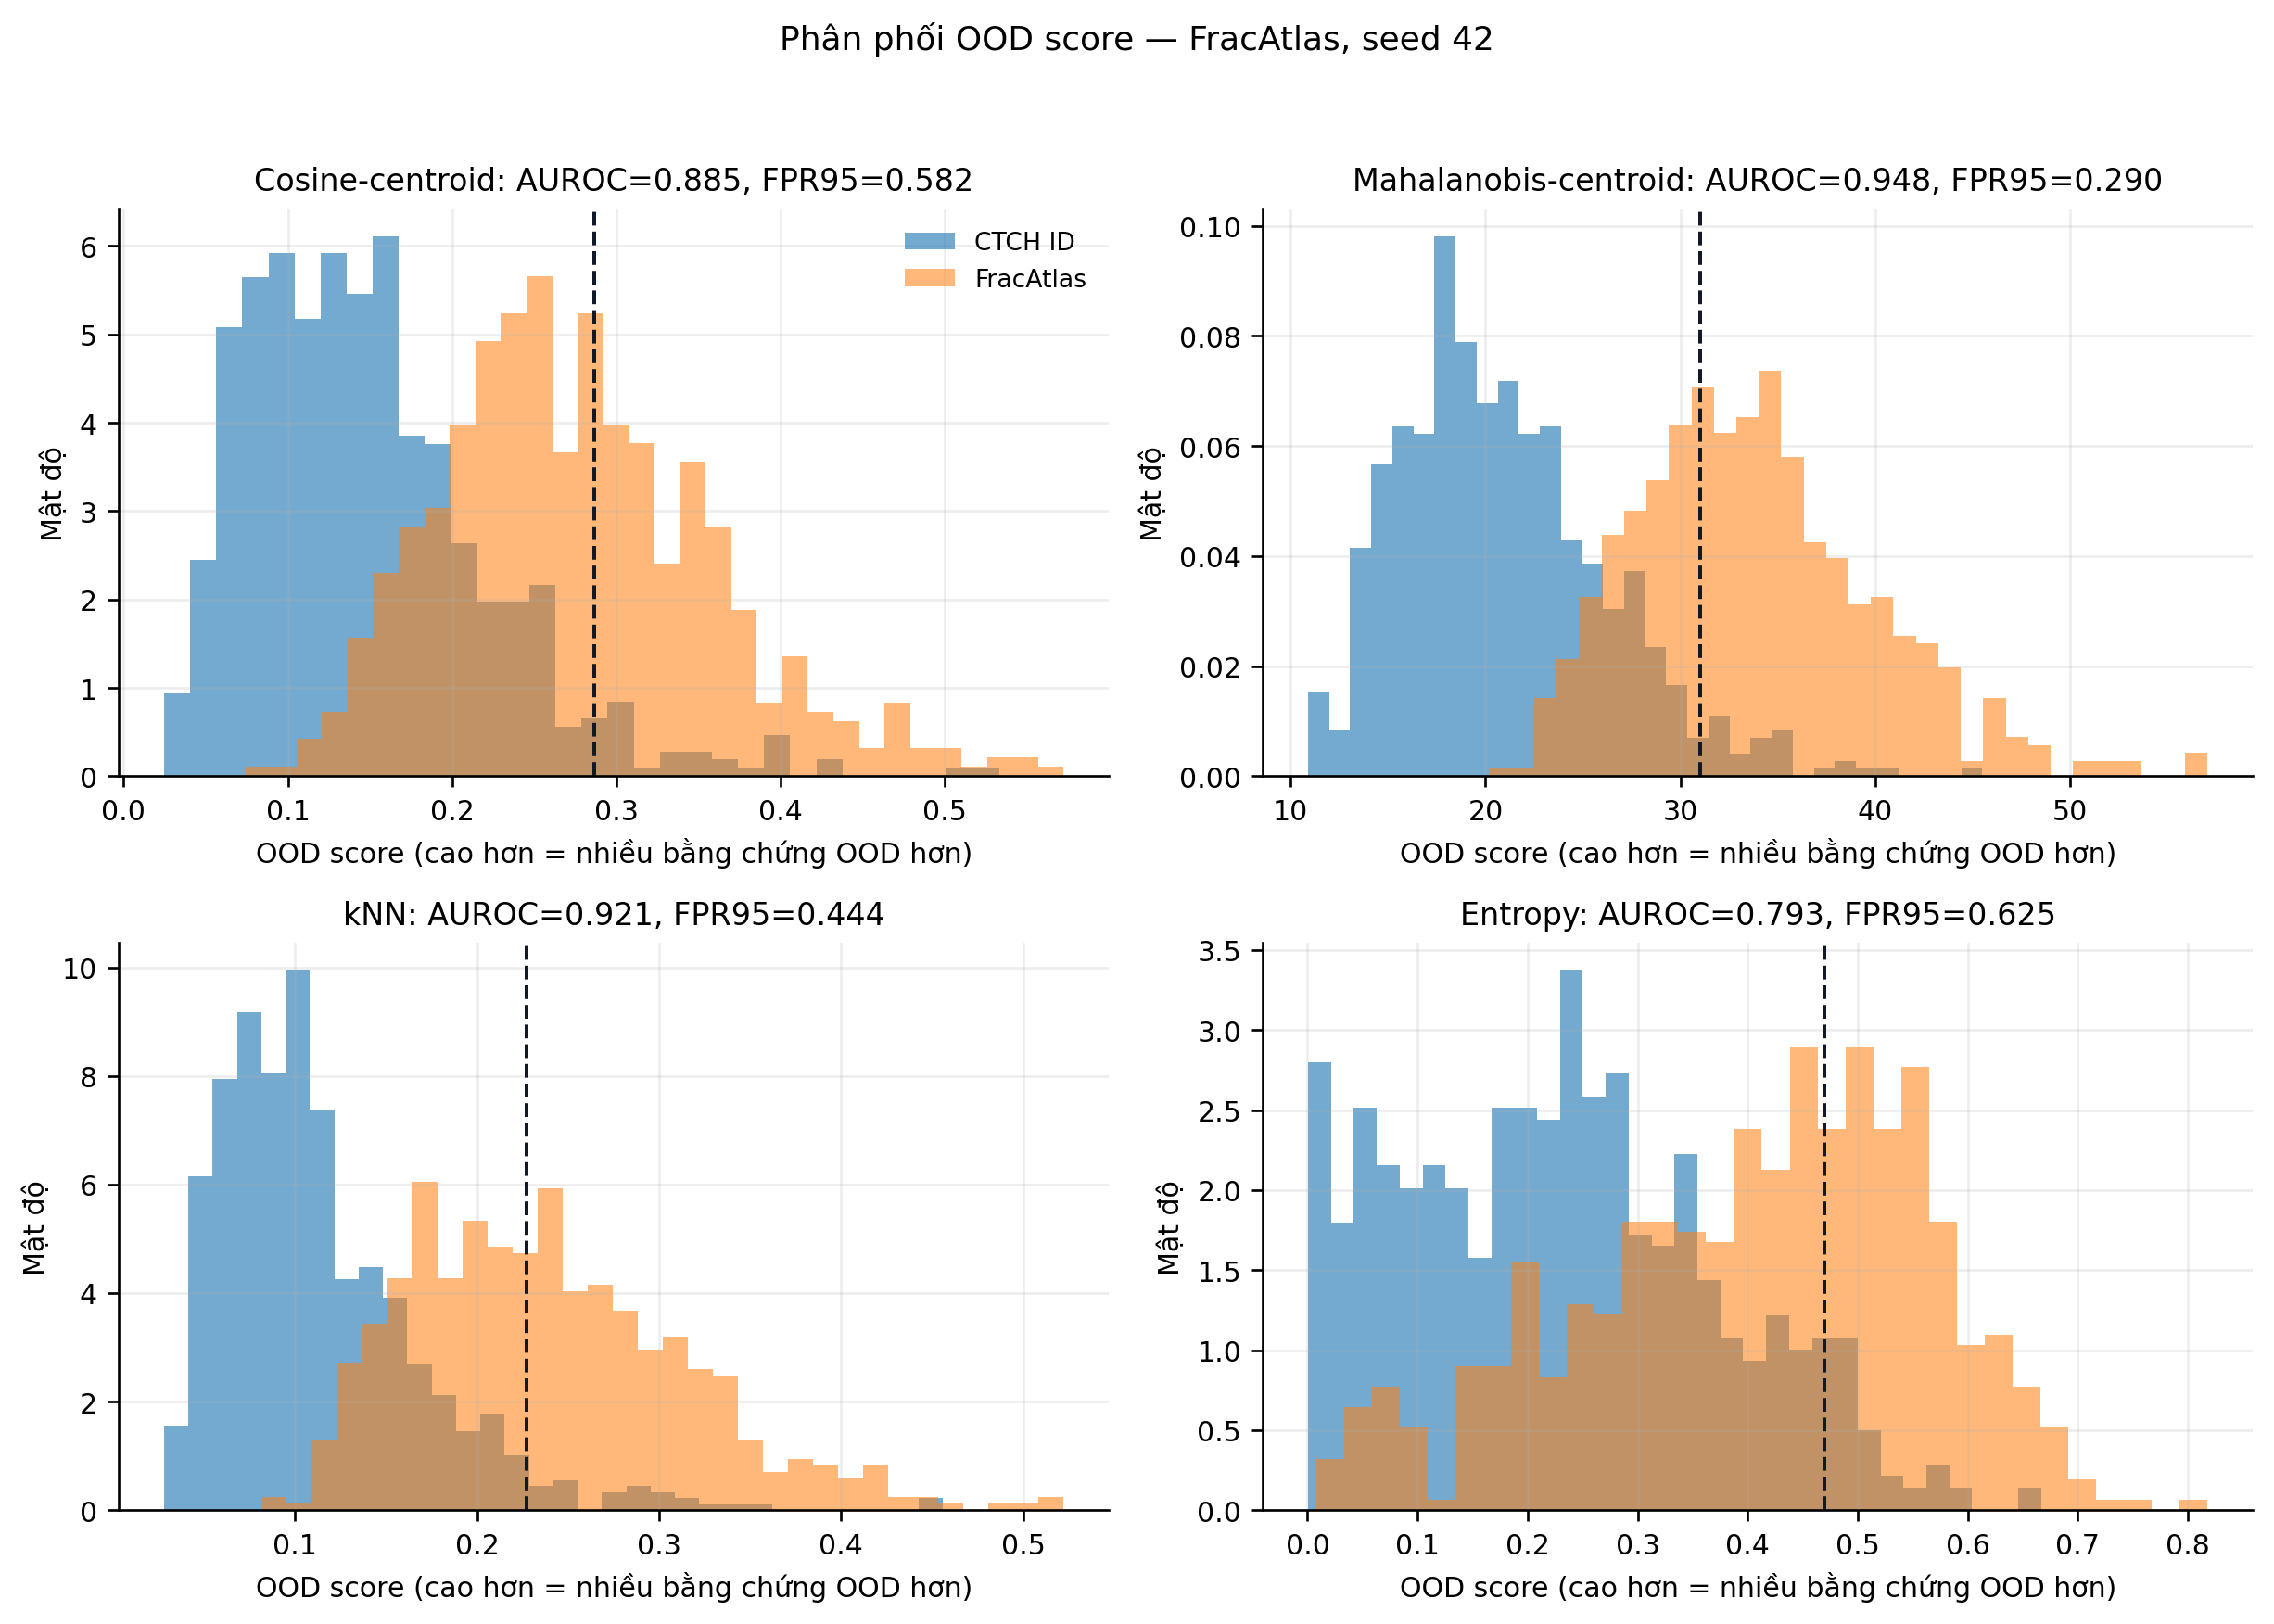
\includegraphics[width=\textwidth]{images/chapter4_draft/appendix/ood_distribution_domain_ood.png}
\caption{Phân phối score của FracAtlas domain OOD và CTCH-ID tại seed 42}
\label{fig:app_ch4_ood_fracatlas}
\end{figure}

\begin{figure}[H]
\centering
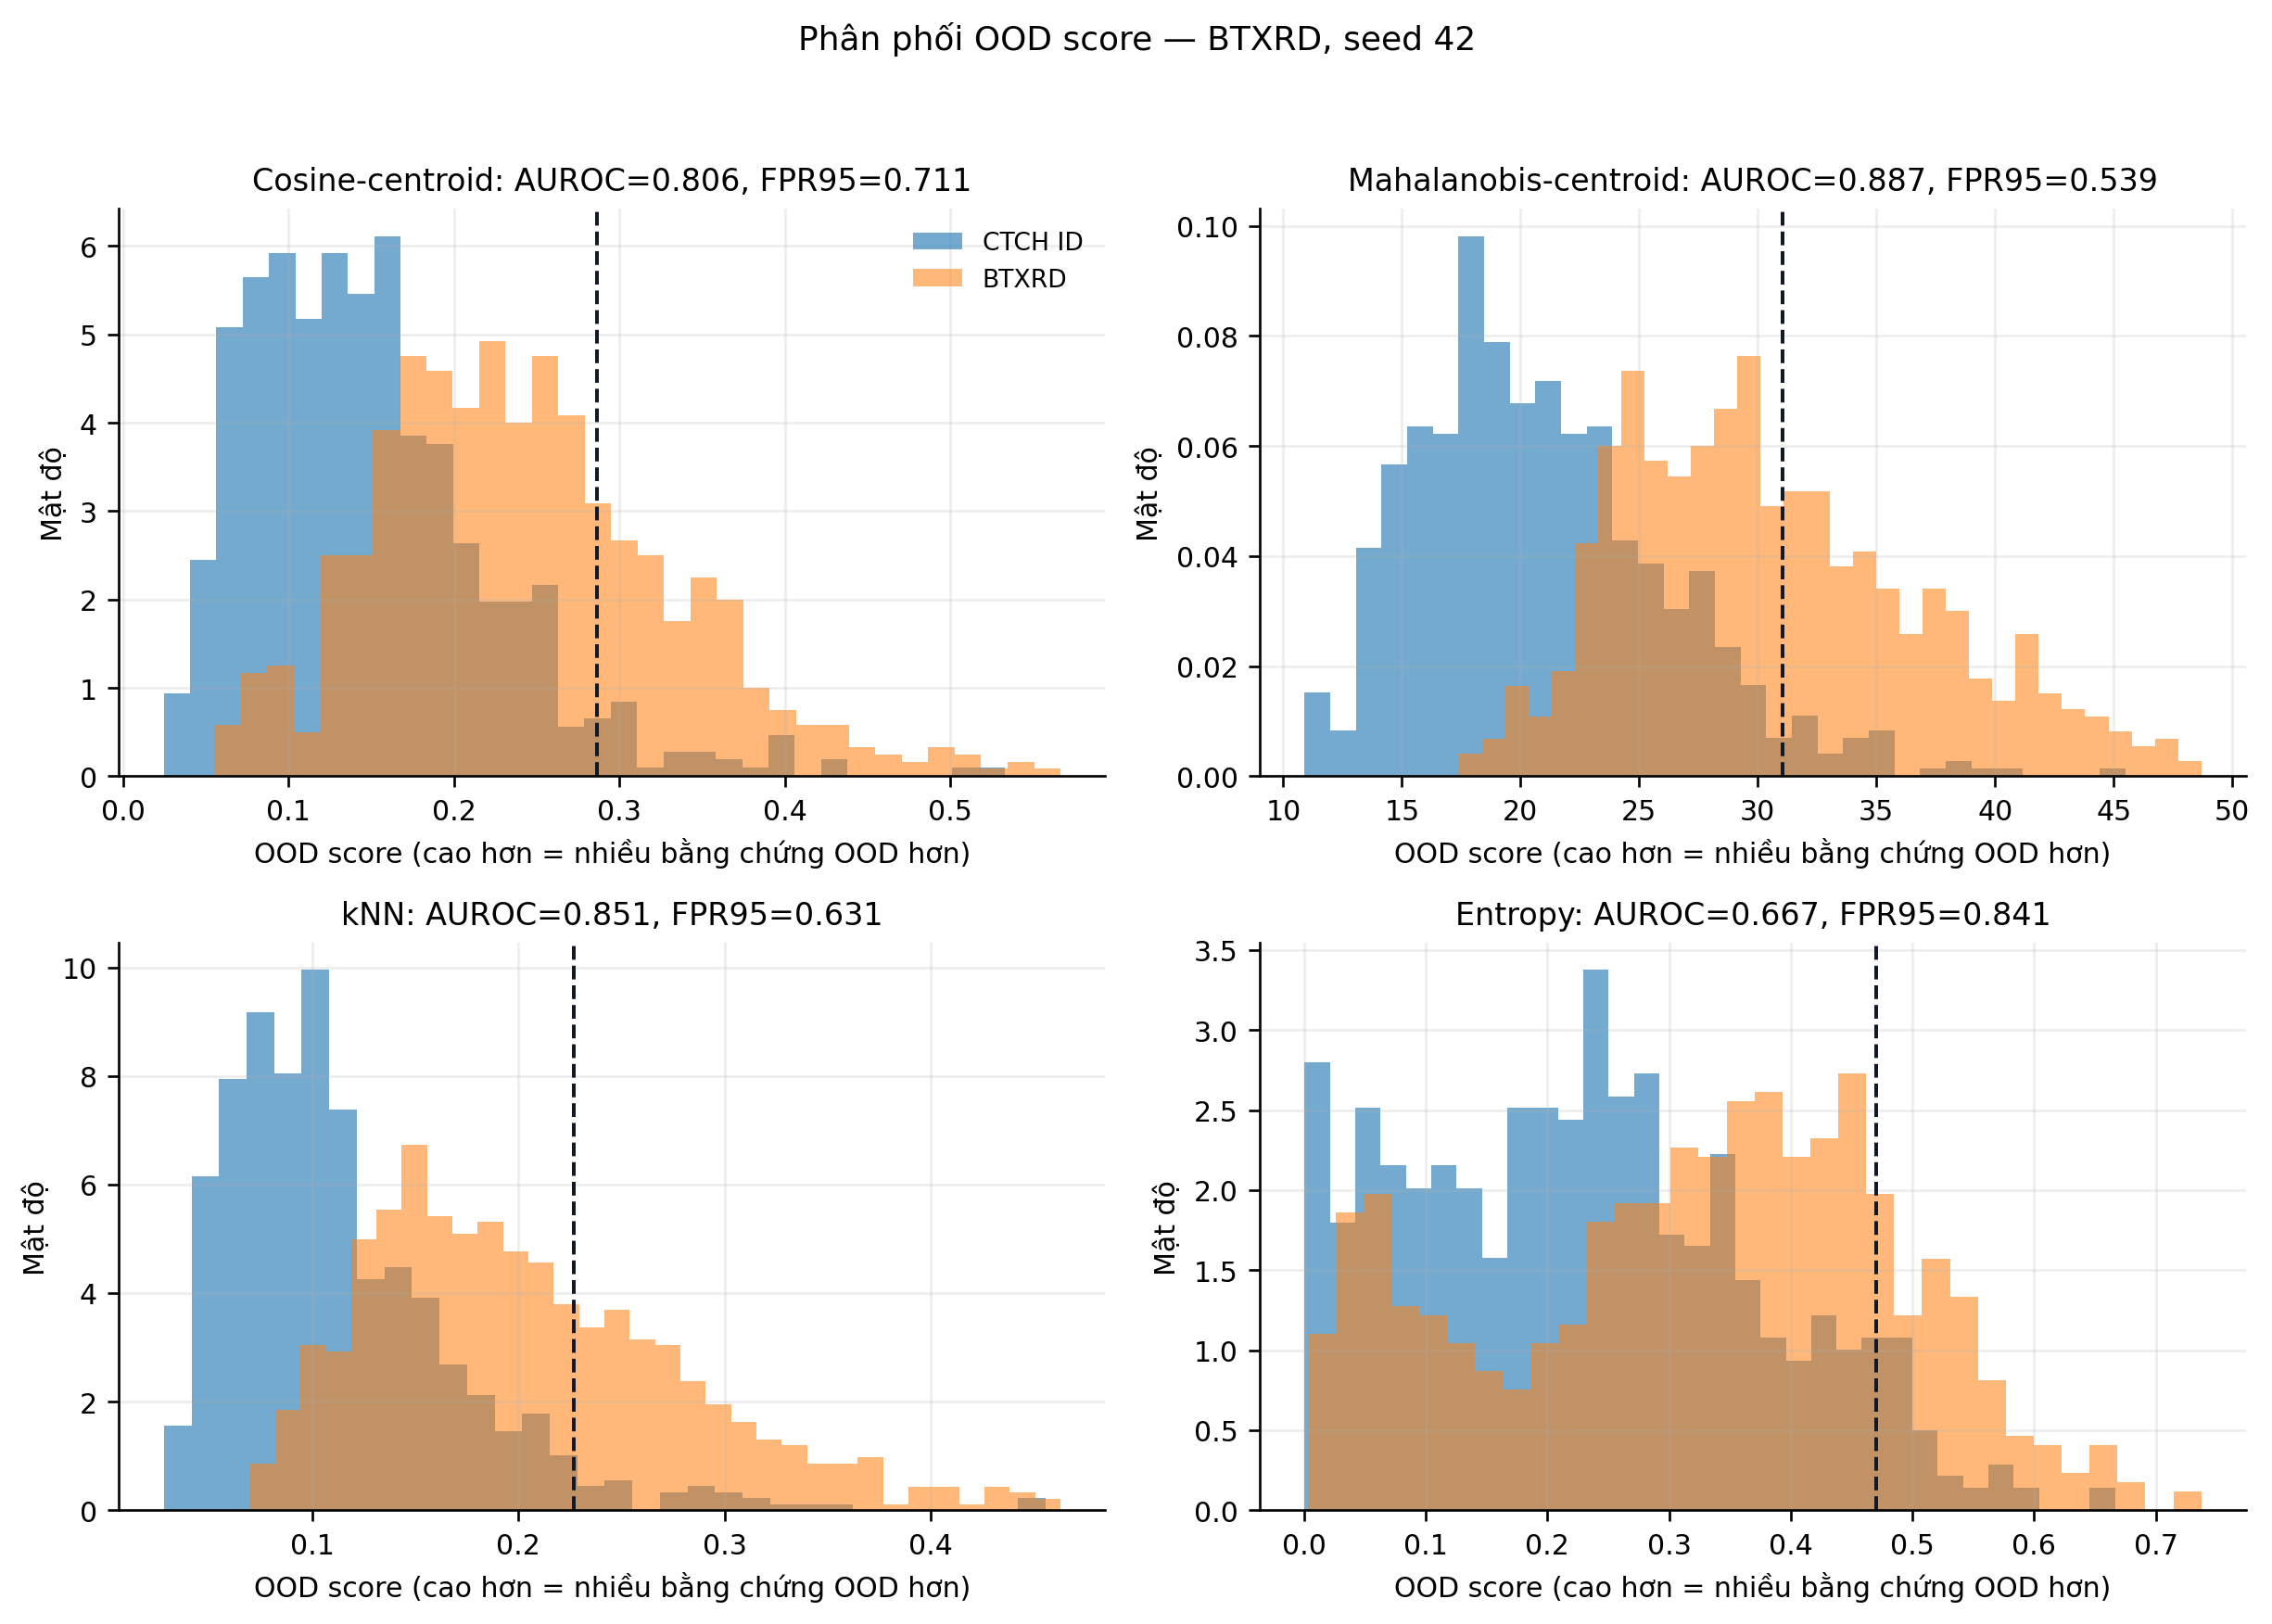
\includegraphics[width=\textwidth]{images/chapter4_draft/appendix/ood_distribution_domain_ood_btxrd.png}
\caption{Phân phối score của BTXRD domain OOD và CTCH-ID tại seed 42}
\label{fig:app_ch4_ood_btxrd}
\end{figure}

\begin{figure}[H]
\centering
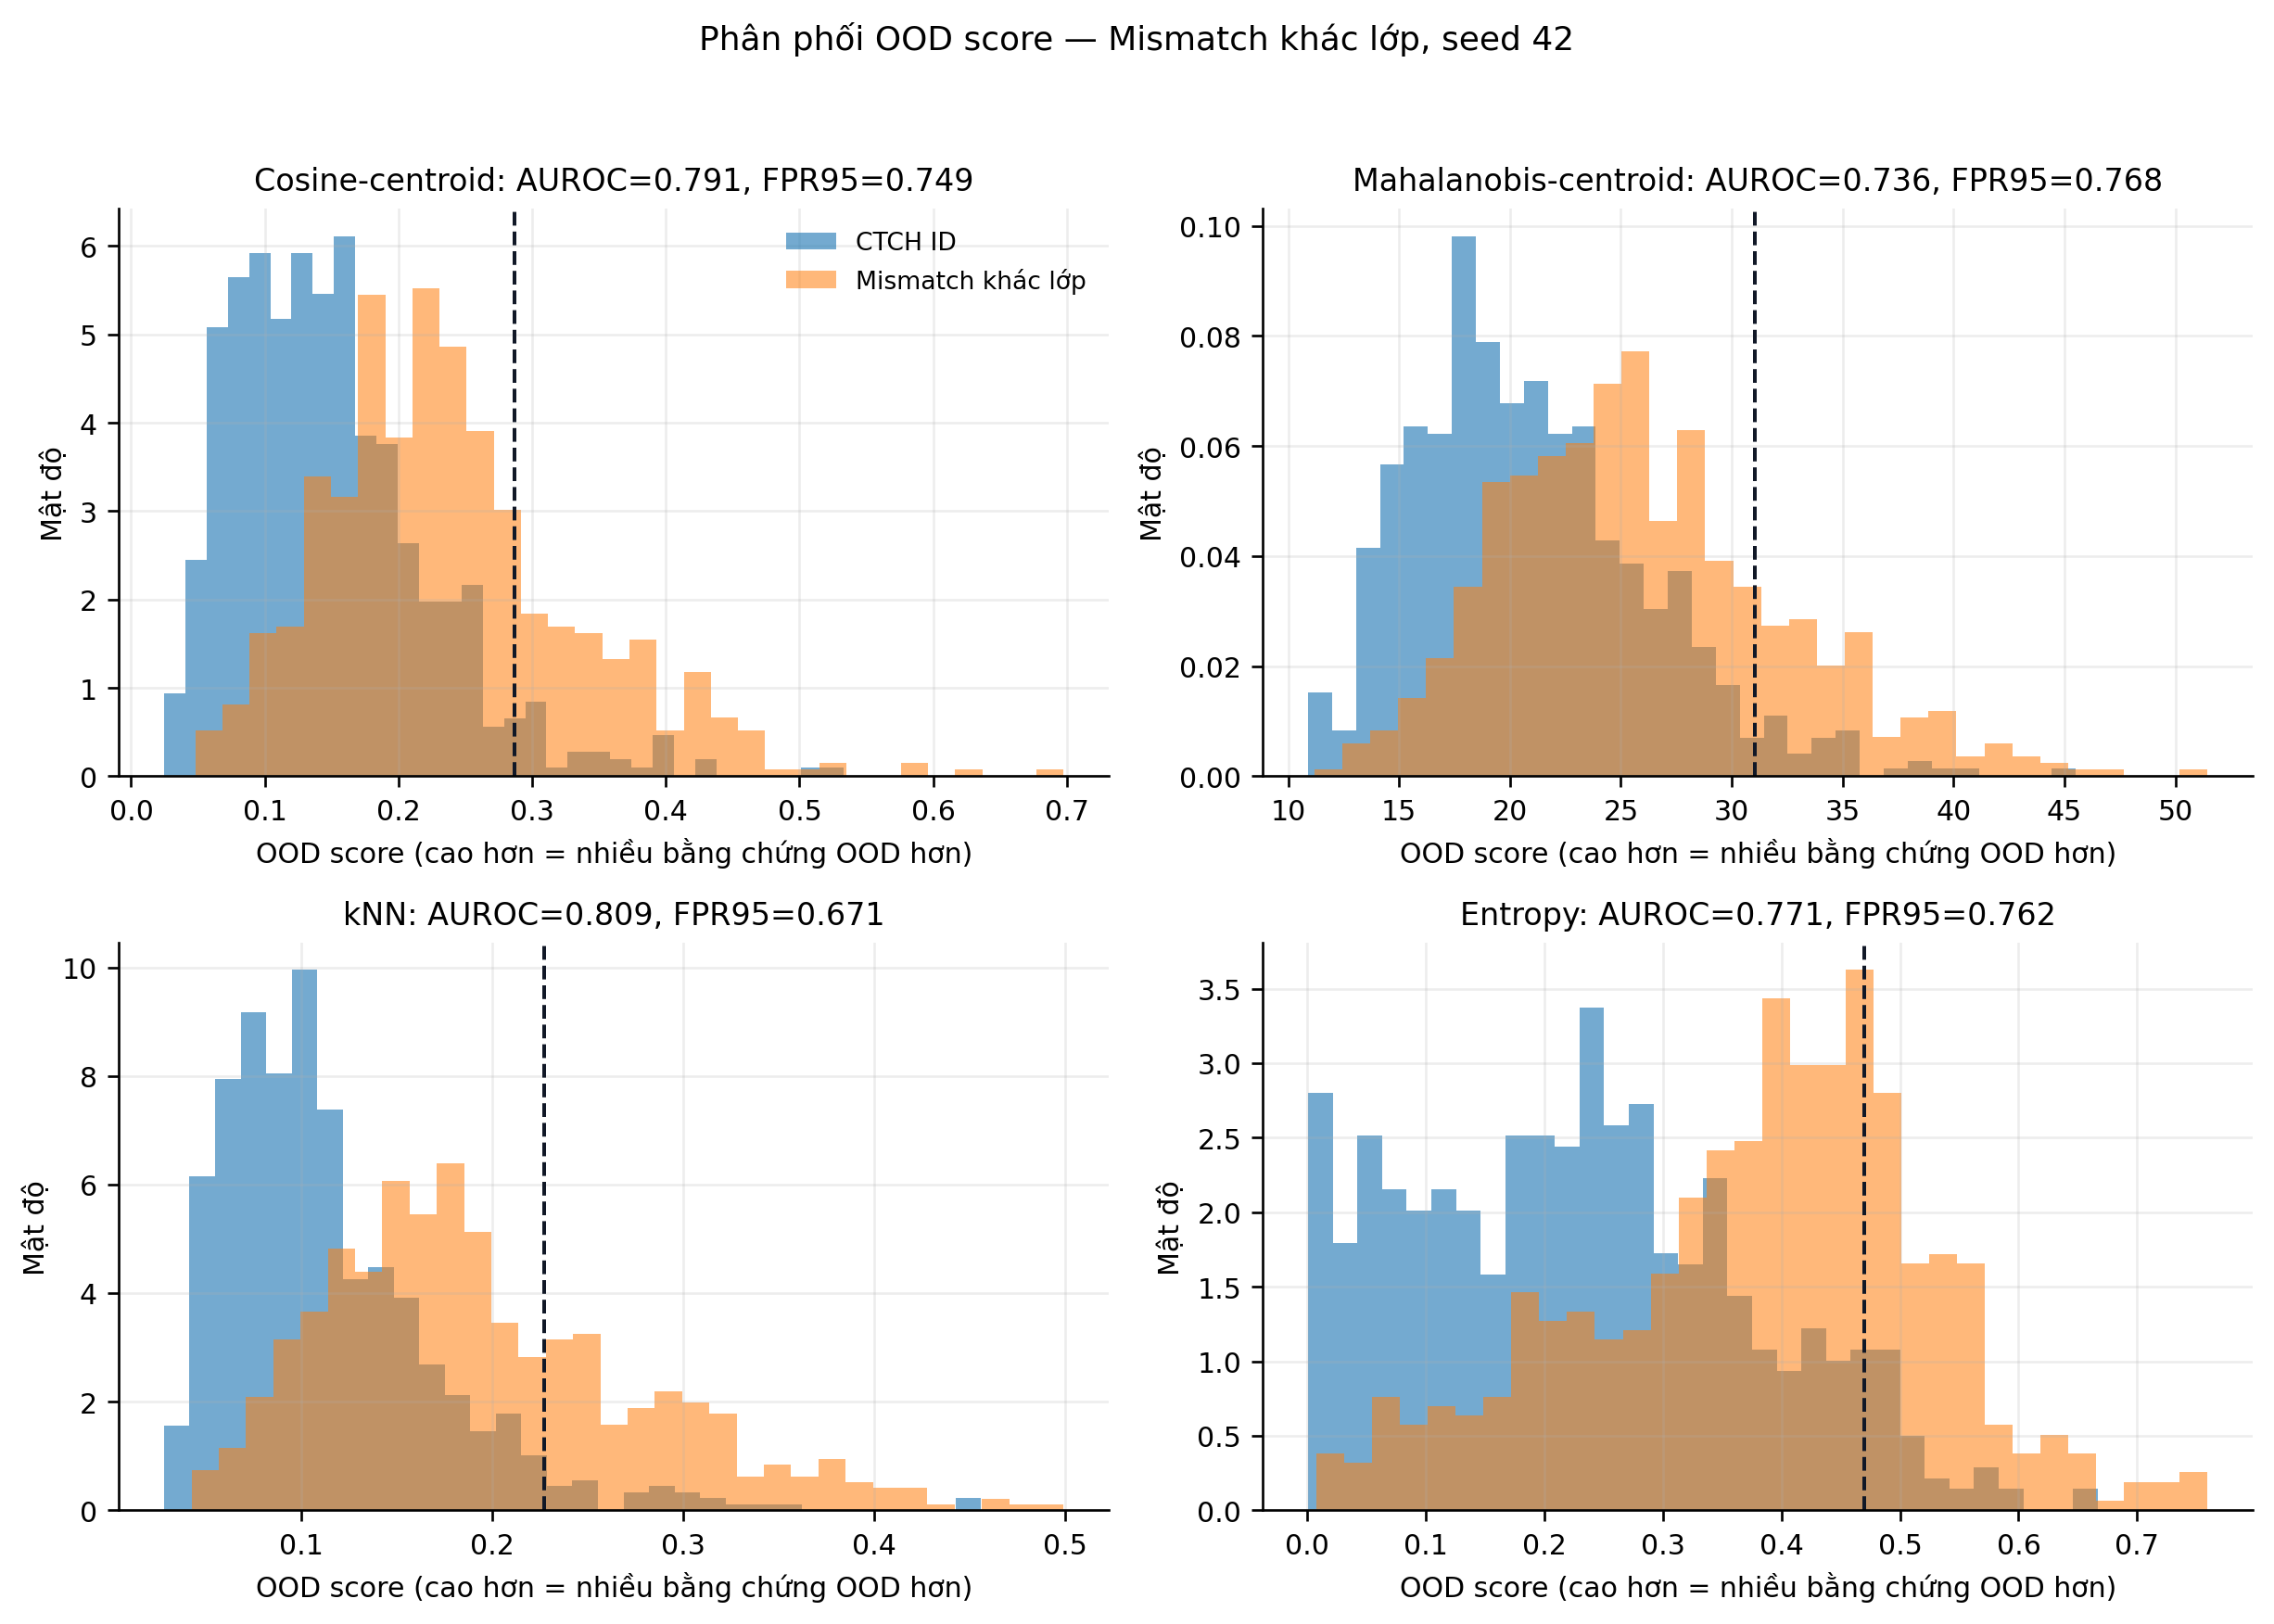
\includegraphics[width=\textwidth]{images/chapter4_draft/appendix/ood_distribution_report_mismatch_cross_class.png}
\caption{Phân phối score của mismatch ảnh--bệnh sử khác lớp và CTCH-ID tại seed 42}
\label{fig:app_ch4_ood_cross}
\end{figure}

\begin{figure}[H]
\centering
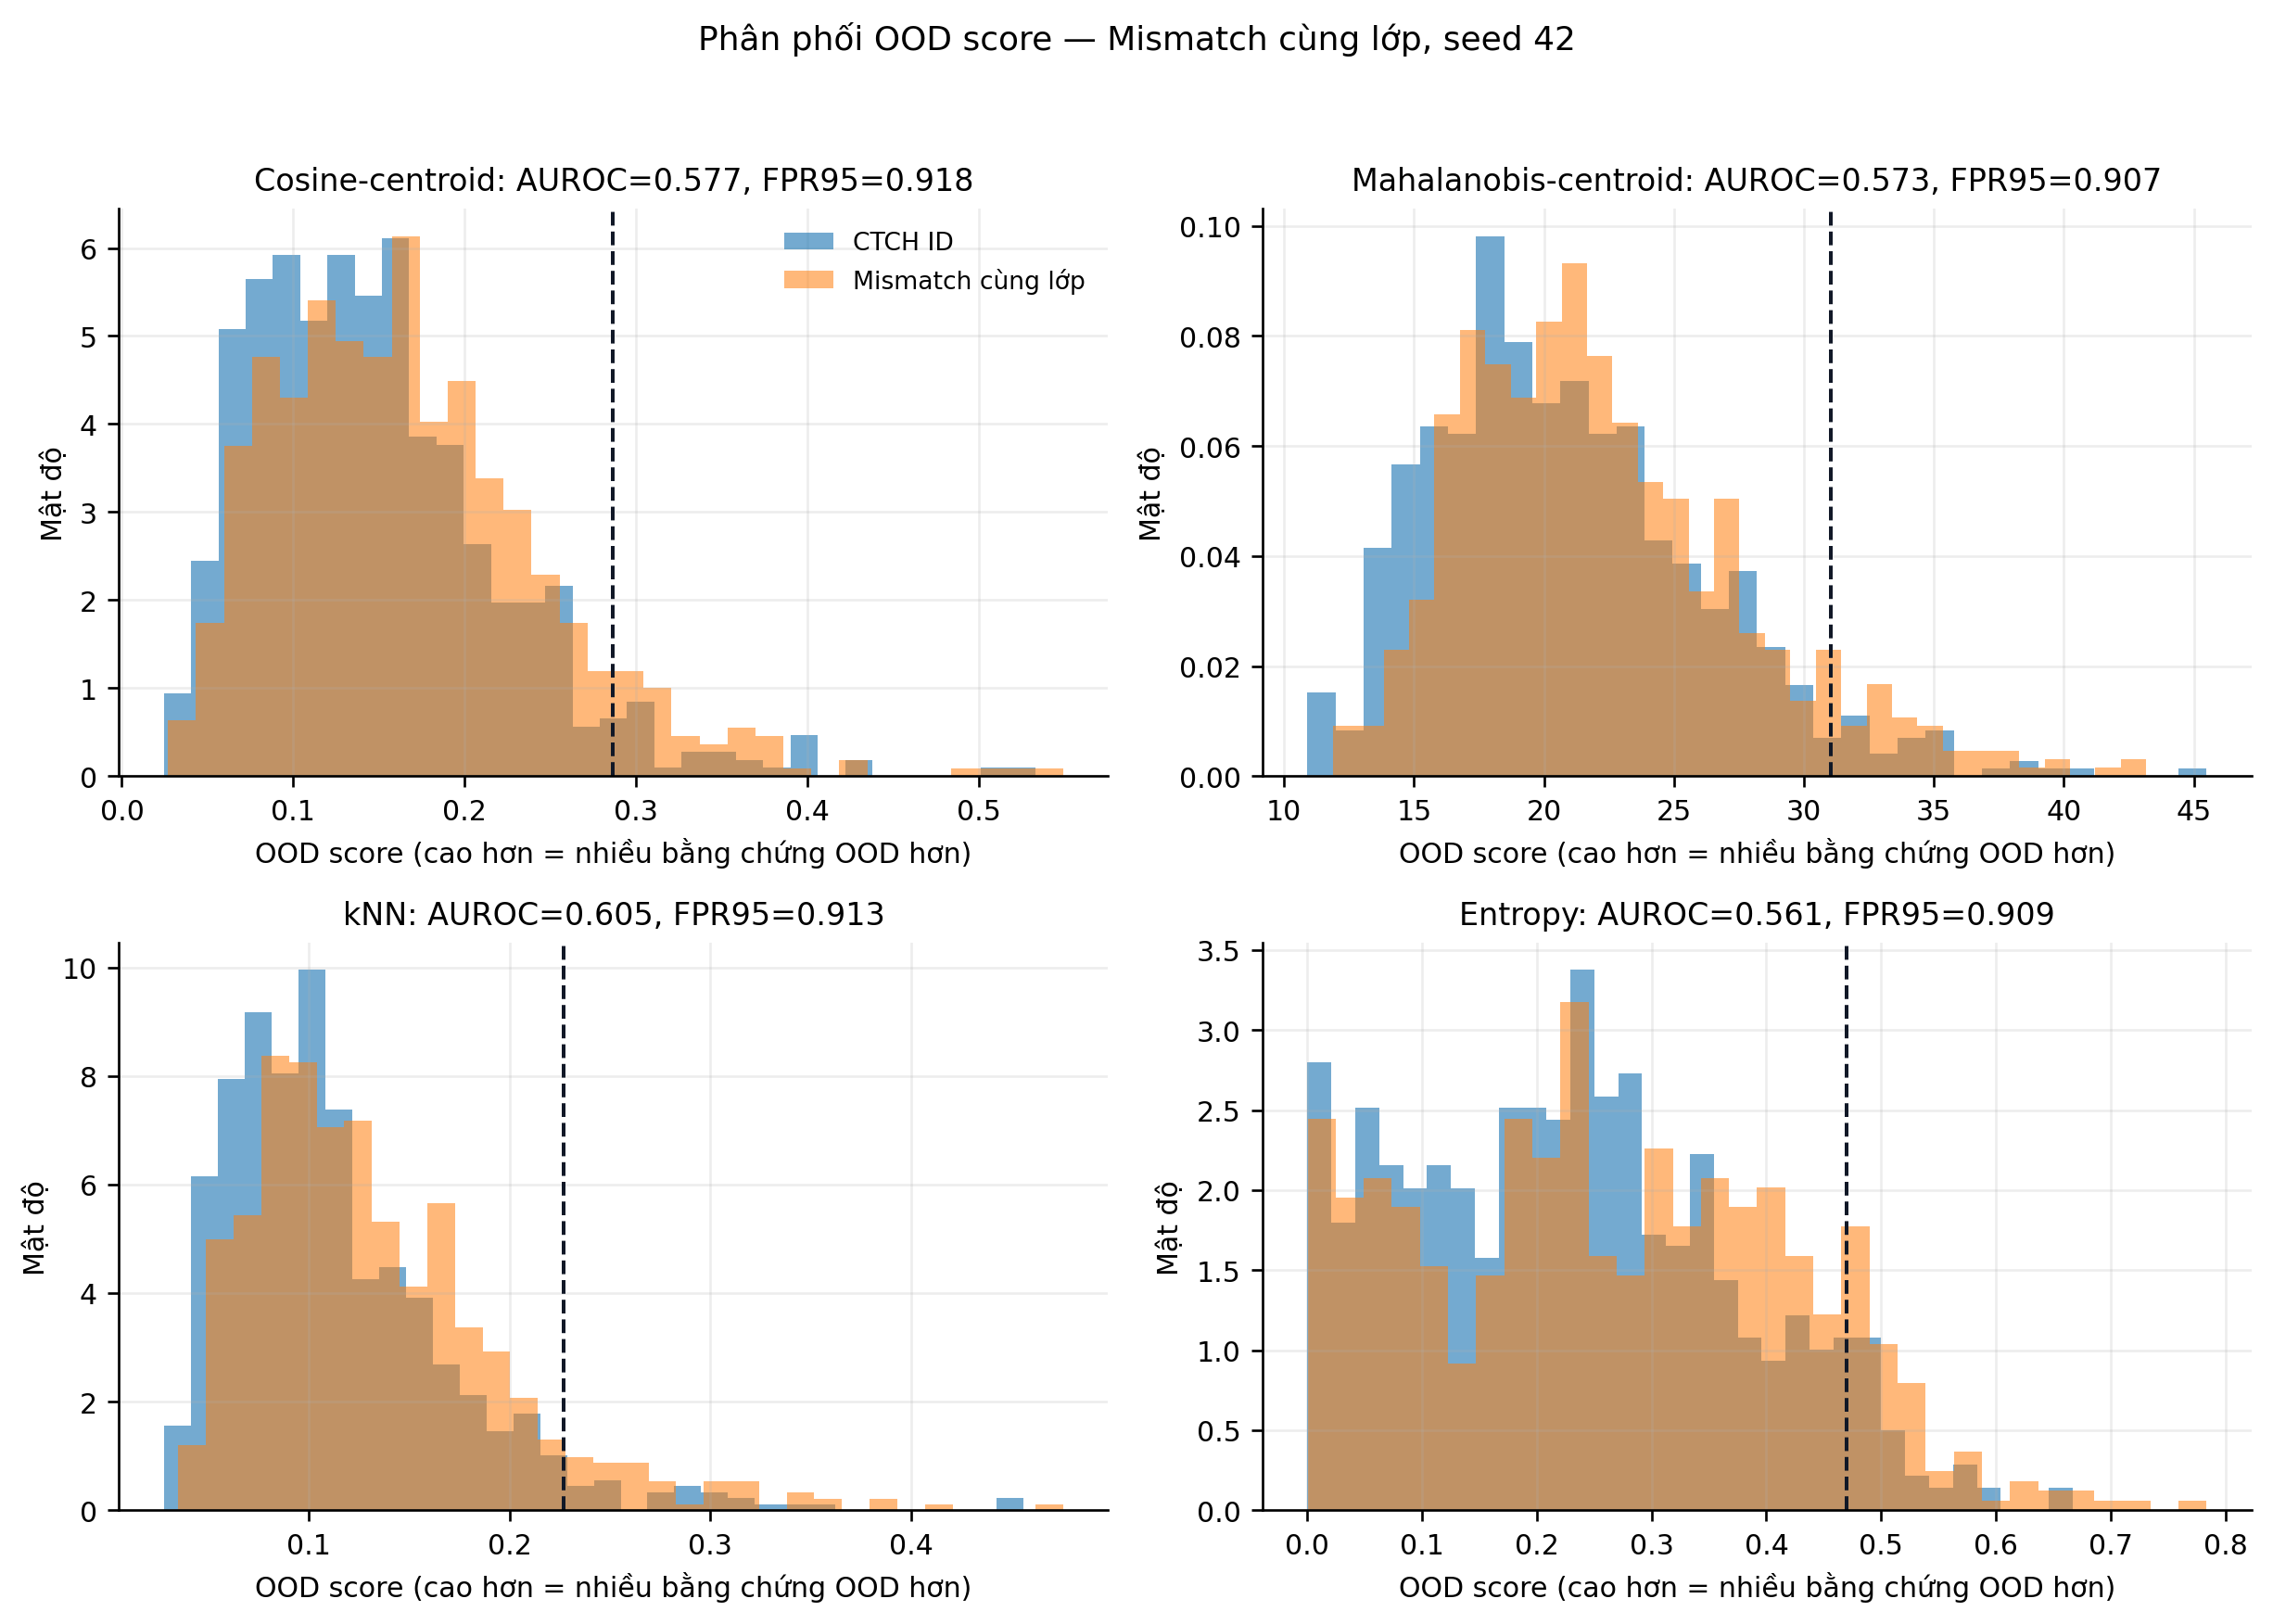
\includegraphics[width=\textwidth]{images/chapter4_draft/appendix/ood_distribution_report_mismatch_same_class.png}
\caption{Phân phối score của mismatch ảnh--bệnh sử cùng lớp và CTCH-ID tại seed 42}
\label{fig:app_ch4_ood_same}
\end{figure}

Các đồ thị cho thấy mức chồng lấn giữa ID và OOD thay đổi theo kịch bản và theo score. Domain OOD tạo dịch chuyển phân phối rõ hơn mismatch cùng lớp; kết quả này phù hợp với AUROC-OOD và FPR@95\%TPR trong phần chính. Đường ngưỡng được lấy từ CTCH validation-ID và giữ cố định khi vẽ tập kiểm thử, nhờ đó các đồ thị không sử dụng nhãn OOD để lựa chọn điểm vận hành.

\section{Hình học không gian biểu diễn}

\begin{figure}[H]
\centering
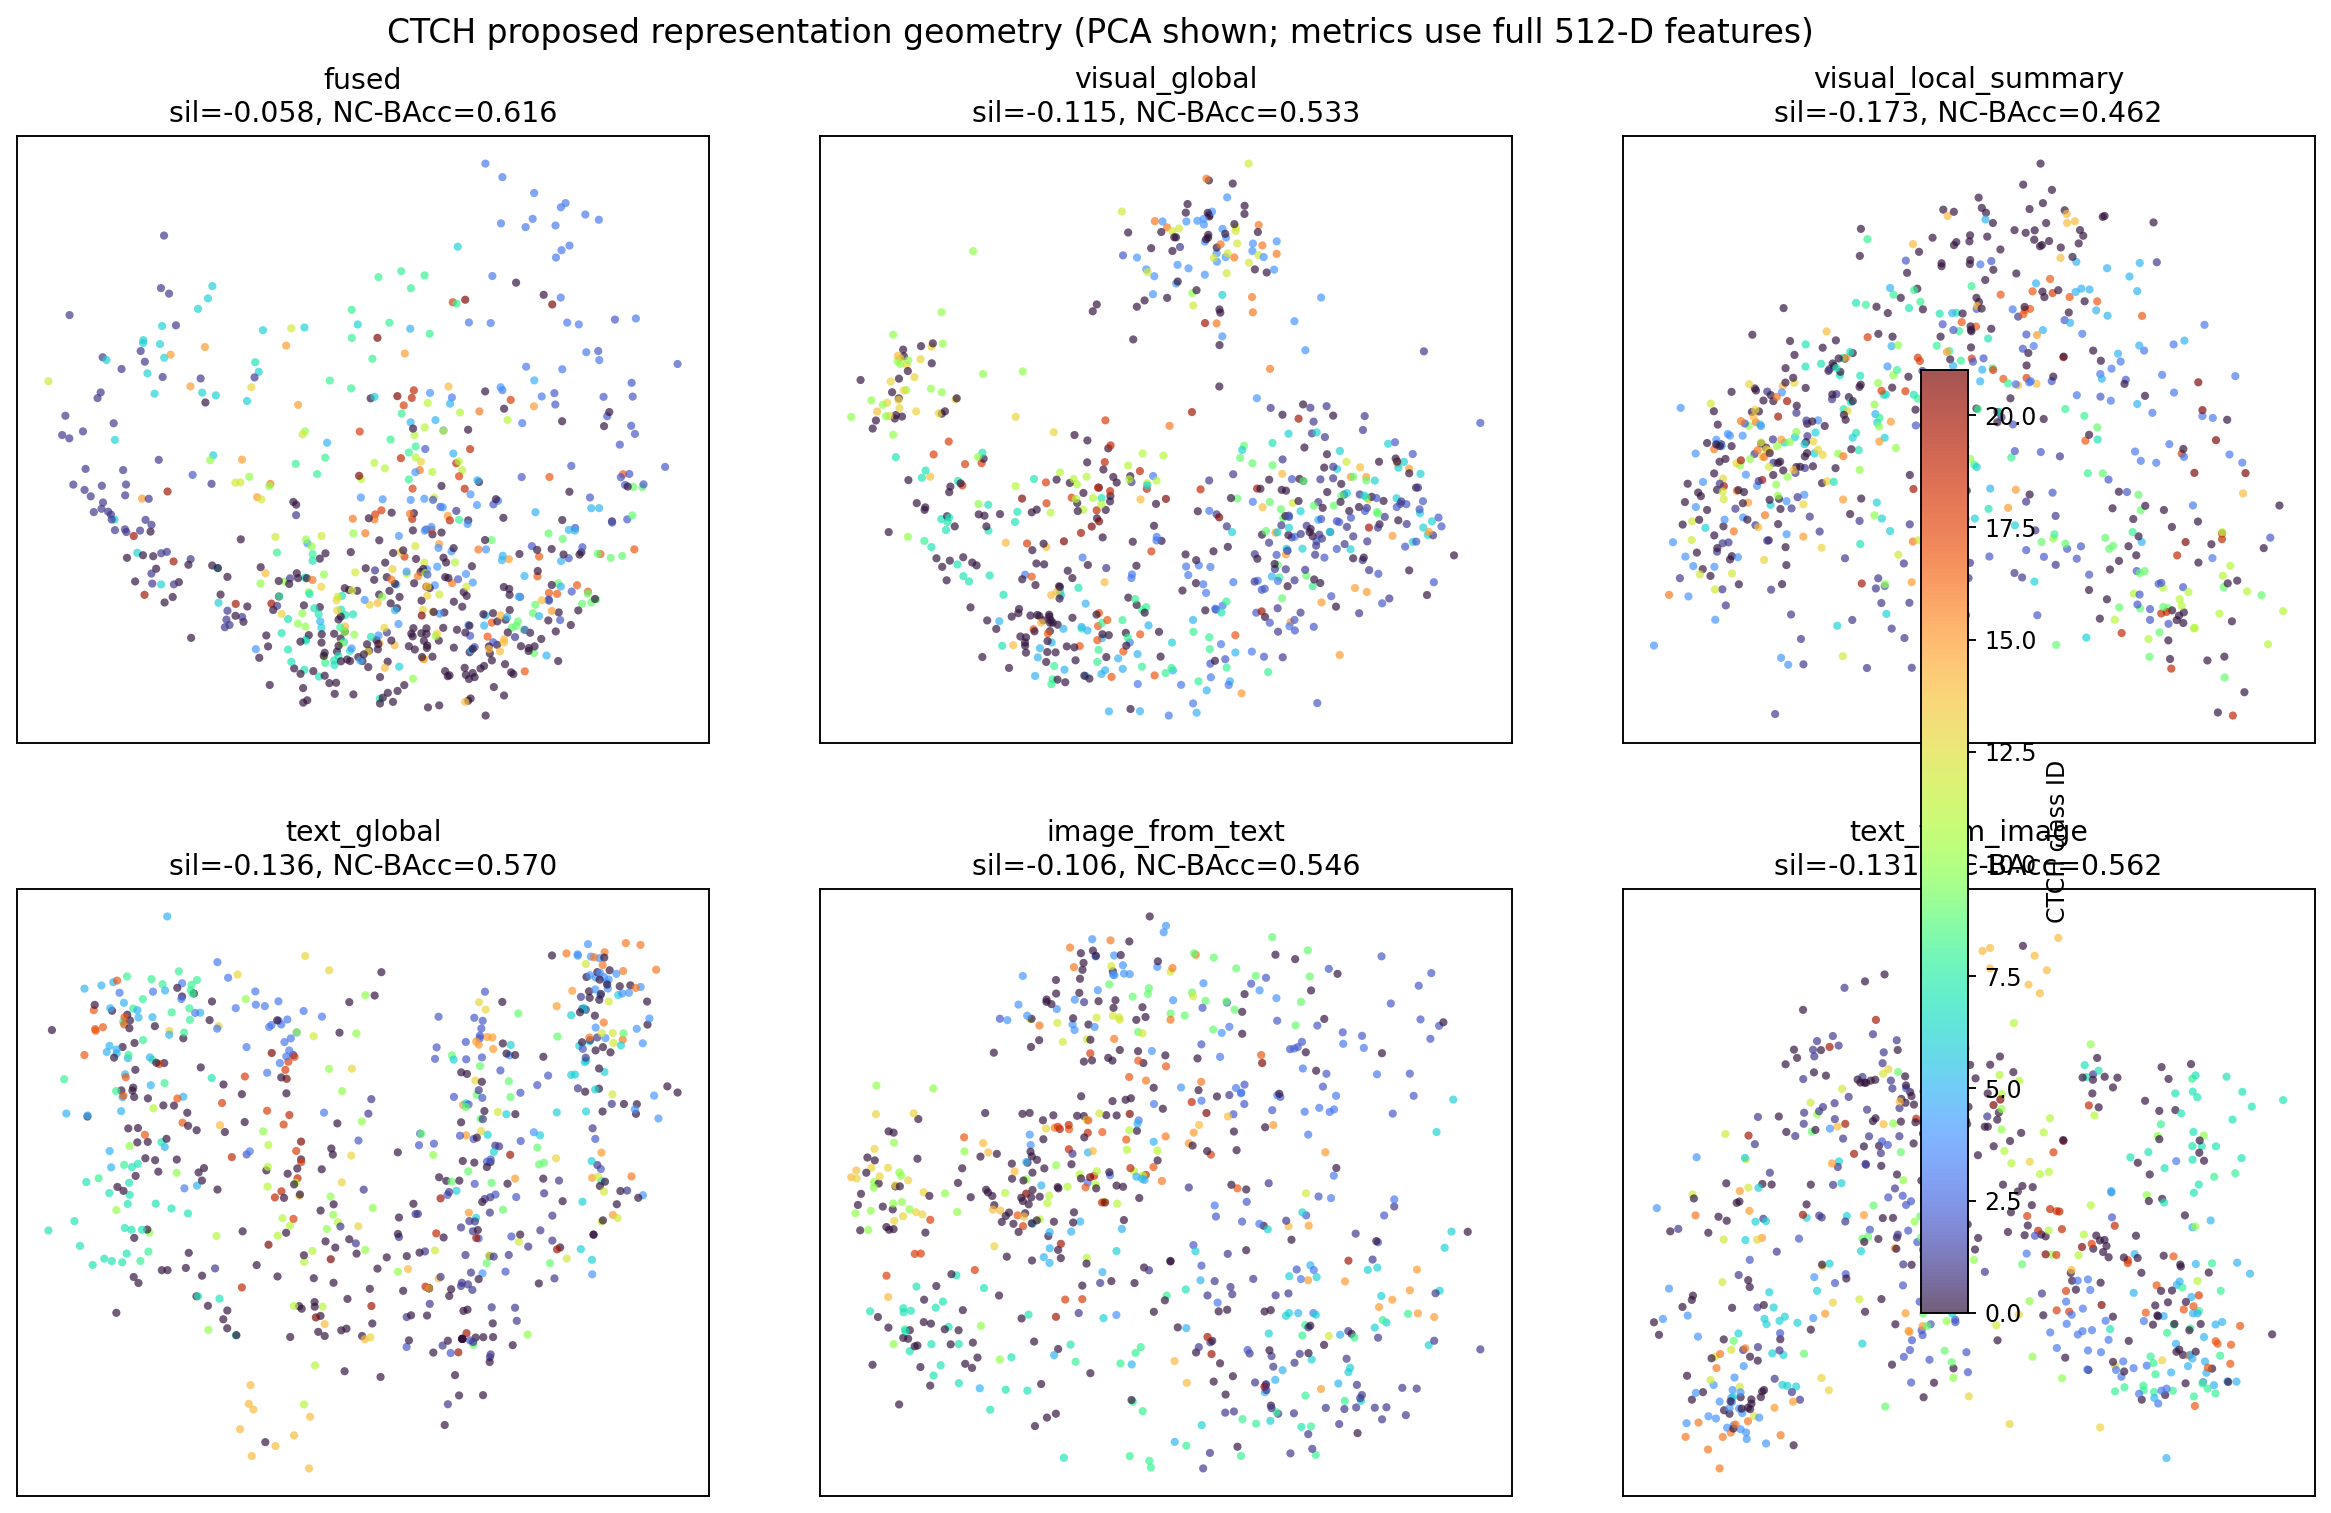
\includegraphics[width=\textwidth]{images/chapter4_draft/appendix/representation_overview_seed42.png}
\caption{Chiếu PCA của các không gian biểu diễn XBone-Net trên CTCH, seed 42}
\label{fig:app_ch4_representation}
\end{figure}

Hình chiếu PCA hỗ trợ quan sát định tính cấu trúc của fused embedding, visual global embedding, visual local summary embedding và text global embedding. PCA chỉ giữ hai phương sai chính nên không được dùng thay cho các độ đo Silhouette, Davies--Bouldin, NMI và centroid Balanced Accuracy trong không gian gốc. Việc fused embedding có cấu trúc tương đối tốt hơn nhưng vẫn chồng lấn giữa nhiều lớp nhất quán với Macro-AUROC cao và Macro-F1 chưa dẫn đầu của mô hình.

\section{Phạm vi báo cáo và khả năng tái tạo}

\begin{table}[H]
\centering
\small
\begin{tabular}{|L{4.0cm}|L{4.0cm}|L{6.1cm}|}
\hline
\textbf{Nhóm kết quả} & \textbf{Phạm vi tổng hợp} & \textbf{Cách sử dụng trong báo cáo} \\ \hline
Zero-shot & Một lần suy luận xác định & Bảng chính, dùng làm mốc trước thích ứng \\ \hline
Full-shot và few-shot & Ba seed 42, 123, 456 & Bảng chính, báo cáo trung bình $\pm$ độ lệch chuẩn \\ \hline
Ablation & Chỉ biến thể có đủ ba seed hợp lệ & Bảng chính; cấu hình suy biến hoặc thiếu seed không được kết luận \\ \hline
OOD & Ba seed, ngưỡng khóa từ validation-ID & Bảng chính; phân phối từng seed đặt ở phụ lục \\ \hline
Attention và representation & Ba seed cho thống kê; seed 42 cho ảnh ca & Thống kê chính và ảnh định tính có ghi rõ seed \\ \hline
ROC, PR và calibration & Một seed minh họa cho mỗi bộ dữ liệu & Phụ lục; không thay thế kết quả tổng hợp \\ \hline
\end{tabular}
\caption{Quy ước sử dụng các đầu ra thực nghiệm hiện có}
\label{tab:app_ch4_reporting_scope}
\end{table}

Mã sinh lại các bảng và hình của bản nháp đọc trực tiếp từ thư mục kết quả hiện có và không huấn luyện lại mô hình. Danh sách đầu vào, hạt giống và đường dẫn đầu ra được lưu cùng thư mục hình để thuận tiện đối chiếu. Khi bổ sung kết quả mới, cần tạo lại toàn bộ bảng tổng hợp để bảo đảm cách in đậm và thứ hạng được cập nhật đồng nhất.
